In questo capitolo verrà descritto lo stato attuale degli strumenti e delle tecnologie correlate a questo elaborato di tesi, partendo da concetti generici come il Cloud e l'Internet of Things fino ad arrivare a soluzioni specifiche come WebAssembly e Kubernetes.

\section{Cloud Computing}

Il concetto di Cloud fu introdotto nel 2006 da Eric Schmidt, in quel momento CEO di Google, in questo modo:\\\\
\say{\textit{Si parte dalla premessa che i servizi e l’architettura per i dati dovrebbero essere sui server. Lo chiamiamo cloud computing perché i dati dovrebbero risiedere in una "nuvola" da qualche parte. E se si possiede il giusto tipo di browser o il giusto tipo di accesso, non importa se si ha un PC o un Mac, un telefono cellulare o dispositivi ancora da sviluppare, si può avere sempre accesso al cloud.}}\\

In sostanza il Cloud Computing\cite{Pallis2010Cloud} è un nuovo paradigma che consiste in un approccio più flessibile basato su risorse condivise e distribuite dai Cloud Providers, cioè le aziende che possiedono i datacenter che si occupano di mantenere l'infrastruttura.\\
Le aziende non sono più obbligate a investire in una infrastruttura privata e mantenerla (con costi aggiunti se si vuole anche ridondanza, scalabilità e distribuzione sul territorio), si affidano invece a dei servizi Cloud che offrono un'interfaccia per deployare applicazioni, creare macchine virtuali o utilizzare direttamente servizi gestiti con una modalità pay-per-use, rendendo l'opzione accessibile anche da piccole aziende con pochi fondi. 

\subsection{Tecnologie Cloud}

Generalmente l'offerta dei Cloud Provider si divide in tre modelli di servizio\cite{Khurana2013Comparison}:
\begin{itemize}

    \item \textbf{IaaS} -- \texttt{Infrastracture as a Service}: mette a disposizione risorse infrastrutturali virtualizzate, come server, storage e reti, e gli strumenti per gestirle. Questo consente agli utenti di gestire sistemi operativi e applicazioni in modo flessibile e autonomo ma senza investire in un'infrastruttura privata. Esempi includono Amazon EC2, Microsoft Azure e Google Compute Engine.
    
    \item \textbf{PaaS} -- \texttt{Platform as a Service}: offre un ambiente di sviluppo e distribuzione di applicazioni, fornendo strumenti, database e middleware senza dover gestire l'infrastruttura sottostante. In questa categoria rientrano prodotti come EKS (Elastic Kubernetes Service), Openshift e Cloud Foundry.

    \item \textbf{SaaS} -- \texttt{Software as a Service}: fornisce applicazioni software accessibili via internet, la responsabilità di installazione e mantenimento dell'applicazione è interamente del Cloud Provider. Esempi comuni sono Google Workspace, Microsoft 365 e Salesforce.
\end{itemize}

Nella Figura \ref{fig:cloud_structure} si può notare come, man mano che si scende nella lista, la responsabilità dell'installazione e del mantenimento dei sistemi si sposti verso il provider.\\ Questo business model strutturato a livelli fa sì che gli ambienti Cloud risultino interessanti sia per chi vuole un'infrastruttura ad alta affidabilità, performante ma gestita in autonomia (approccio IaaS) che per chi vuole utilizzare un servizio gestito senza preoccuparsi del suo mantenimento (SaaS)\cite{Tsai2014Software-as-a-service}.

\FloatBarrier
\begin{figure}[h]
    \centering
    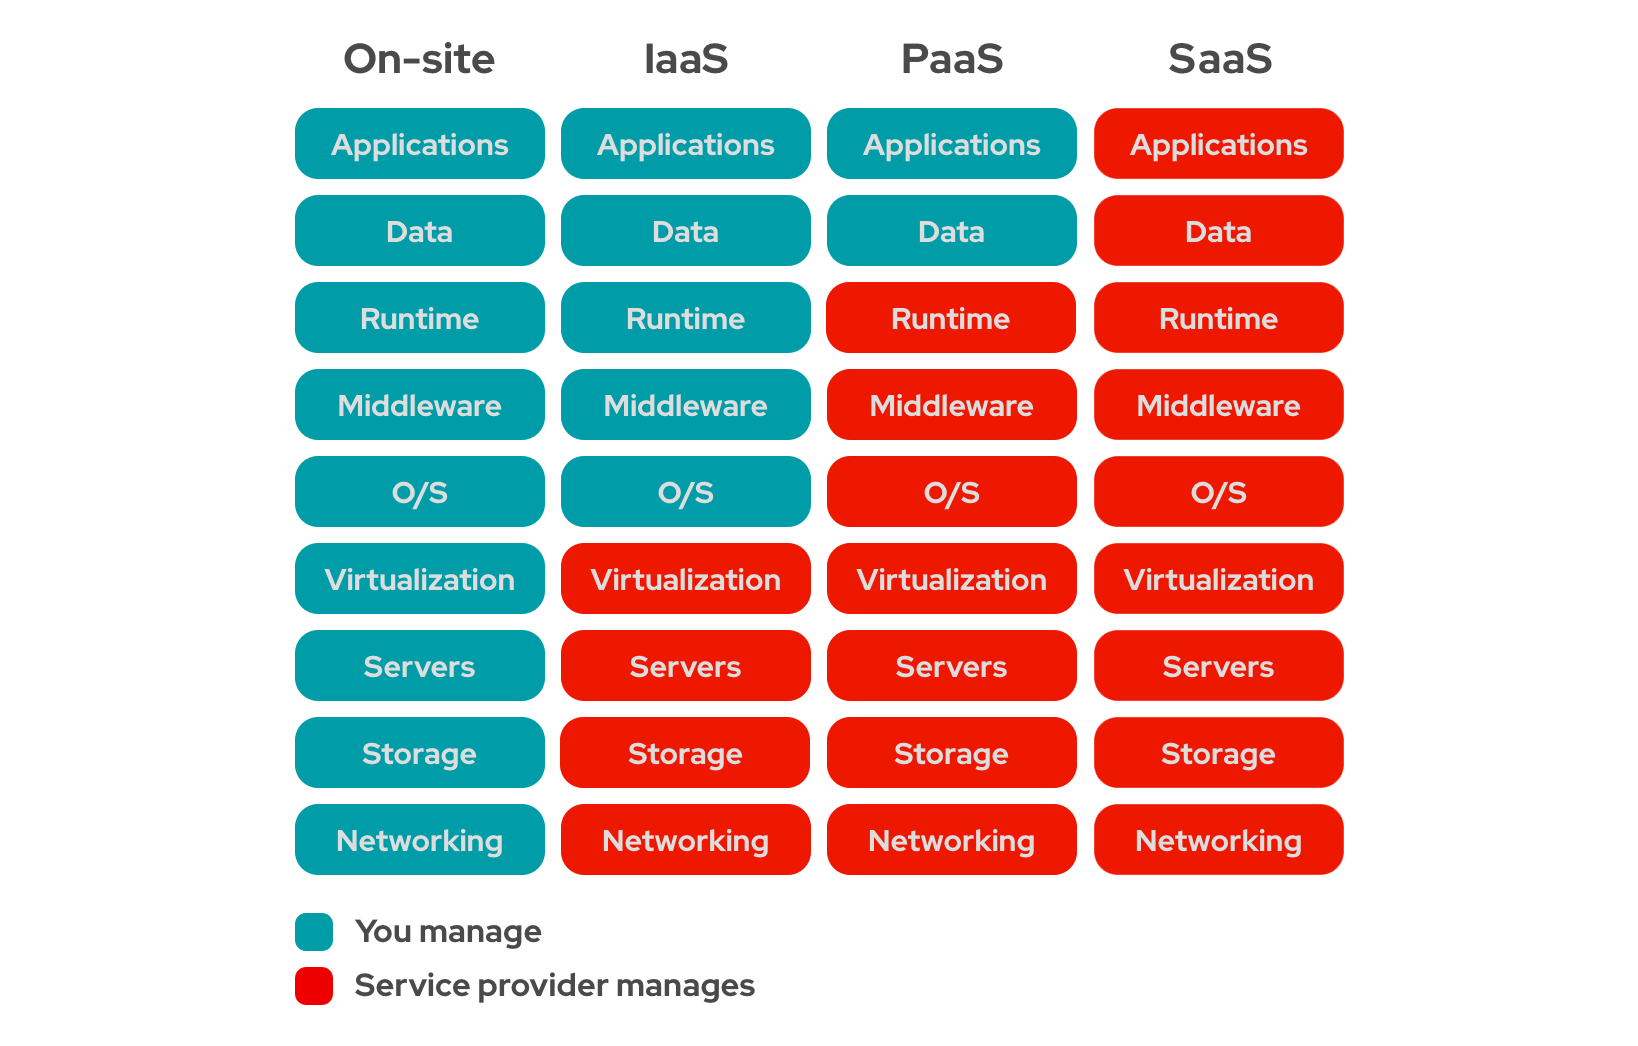
\includegraphics[width=0.75\textwidth]{img/iaas-paas-saas-diagram5.1-1638x1046.png}
    \caption{Cloud Computing e IaaS, PaaS, SaaS\protect\footnotemark}
    \label{fig:cloud_structure}
\end{figure}
\FloatBarrier

\footnotetext{\url{https://www.redhat.com/it/topics/cloud-computing/iaas-vs-paas-vs-saas}}

\subsection{Serverless e FaaS}

Negli ultimi anni il Cloud Computing ha visto una profonda trasformazione con i provider che assumono sempre più il compito della gestione dell’infrastruttura, permettendo così alle aziende di concentrarsi sullo sviluppo della logica di business. Questo spostamento verso modelli simili al SaaS consente agli sviluppatori di dedicarsi principalmente alla creazione di applicazioni innovative, lasciando ai provider la responsabilità della manutenzione e della scalabilità del sistema.\\
Un esempio emblematico di questa evoluzione è rappresentato dal paradigma del Serverless Computing, un modello che si posiziona tra il PaaS e il SaaS. In questo contesto, il codice viene eseguito in risposta a eventi specifici, eliminando la necessità di gestire manualmente server e infrastruttura sottostante. Tale approccio, noto anche come Function as a Service (FaaS), sta rapidamente guadagnando popolarità per la sua semplicità d’uso\cite{Wen2022Rise} e per la capacità di adattarsi dinamicamente alle esigenze delle applicazioni.\\
Adottando soluzioni FaaS, come ad esempio AWS Lambda, le applicazioni web possono eseguire logiche backend senza dover implementare un server dedicato. In questo modo, gli sviluppatori sono in grado di focalizzarsi sulla parte frontend e sulle funzionalità core, mentre la gestione dell’infrastruttura viene delegata al provider. Questo modello porta con sé vantaggi significativi, come una facile scalabilità e costi operativi contenuti, sebbene imponga anche sfide in termini di performance e sicurezza, che richiedono una valutazione accurata\cite{Li2023Serverless}.\\
Questo approccio si differenzia dall'IaaS, che offre il massimo controllo ma richiede una gestione completa dell'infrastruttura, e dal PaaS, che semplifica lo sviluppo a discapito di una maggiore flessibilità. Allo stesso tempo, a differenza del SaaS, che fornisce applicazioni già pronte all'uso, il FaaS consente una personalizzazione più mirata, pur comportando alcune sfide come i ritardi nei ``cold start" (tempo di istanziamento in cloud della funzione)\cite{Yussupov2020FaaSten} e la dipendenza da specifici provider.

\subsection{IoT ed Edge Computing}

\texttt{IoT (Internet of Things)}\cite{Laghari2021A} è un termine diffuso nella comunità IT e si riferisce a quei dispositivi (le ``cose") che sono in grado di connettersi ad internet. I dispositivi collegati forniscono delle metriche che possono essere aggregate, analizzate ed elaborate dai servizi eseguiti in Cloud, dal quale possono essere consultate tramite interfacce grafiche o utilizzate per processi decisionali o perfino per trainare dei modelli di Machine Learning.\\
Attualmente l'implementazione del modello IoT si è assestata in un'architettura composta da tre classi di componenti principali\cite{Sultana2020IoT}:
\begin{itemize}
    \item \textbf{Things}: sensori, attuatori e macchine che forniscono metriche e ricevono comandi, in grado di comunicare con un gateway con protocolli leggeri, tipicamente poco sicuri e con bassa QoS.
    \item \textbf{IoT Gateway}: sistema installato in loco in grado di comunicare con tutti i dispositivi e stabilire una connessione sicura con i servizi in Cloud. Consente anche di effettuare semplici operazioni sui dati, come aggregazioni e batching. Un esempio di gateway potrebbe essere uno smartphone, che raccoglie dati dai sensori e li sincronizza con applicazioni situate in Cloud [\ref{fig:iot}].
    \item \textbf{Servizi Cloud}: servizi disponibili sul Cloud che possono fornire molte funzionalità, fra cui
    \begin{itemize}
        \item Sistemi di processing dei dati in real time, come Apache Kafka o servizi FaaS
        \item Algoritmi di training per modelli di Machine Learning
        \item Dashboard per visualizzare le metriche dei sensori
    \end{itemize}
\end{itemize}

Un esempio comune di questa suddivisione è il nostro smartphone: esso raccoglie delle metriche tramite dei sensori (posizione, contatore dei passi etc), le aggrega e le sincronizza con applicazioni situate in Cloud, fungendo di fatto da IoT Gateway. Questo esempio viene illustrato nella Figura \ref{fig:iot}.

\FloatBarrier
\begin{figure}[h]
    \centering
    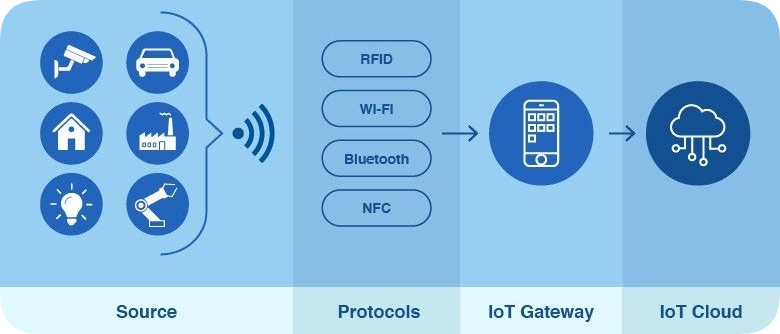
\includegraphics[width=0.8\textwidth]{img/IoT-app.png}
    \caption{Smartphone come IoT Gateway\protect\footnotemark}
    \label{fig:iot}
\end{figure}
\FloatBarrier

\footnotetext{\url{https://elainnovation.com/en/mobile-as-a-gateway-iot/}}

Sebbene questo approccio porti una notevole evoluzione rispetto all'industria tradizionale presenta anche qualche svantaggio: innanzitutto spostare tutto il carico computazionale sul Cloud potrebbe portare a costi elevati nel lungo termine, specialmente se il numero di dispositivi da gestire aumenta\cite{Barcelo2016IoT-Cloud}.\\
Un altro problema non trascurabile è quello della latenza, infatti certe operazioni potrebbero essere time-critical per i dispositivi e la comunicazione con dei servizi in Cloud aggiunge inevitabilmente un ritardo considerevole\cite{Shukla2021Improving}.

\subsubsection{Edge Computing}

Per risolvere queste criticità negli ultimi anni si è affermato un nuovo modello, detto Edge o Fog Computing\cite{Hoshikawa2019Edge} (Fog perché non è su una ``nuvola", ma più vicino ai dispositivi). Questo modello consiste nello spostare una buona parte del carico computazionale dal Cloud al dispositivo Edge, che quindi non sarà più un semplice gateway.\\
Il nodo Edge viene infatti potenziato, può supportare la virtualizzazione e l'esecuzione di moduli che possono essere configurati da remoto, così da ridurre la latenza per le operazioni critiche per i dispositivi IoT\cite{Shukla2021Improving}. Le metriche elaborate verranno poi sincronizzate con i servizi in Cloud in modo ottimizzato, così da ridurre i costi.\\
La relazione fra Edge e Cloud diventa una sinergia, un caso d'uso moderno e performante è quello in cui i servizi Cloud trainano modelli di Machine Learning e li inviano poi ai nodi Edge, che li sfruttano per un'esecuzione dei moduli ottimizzata.
L'unico svantaggio dell'approccio Fog Computing rispetto al Cloud tradizionale è il costo aumentato dato dall'investimento iniziale sull'infrastruttura del nodo Edge.\\

\section{Containerizzazione ed orchestrazione}
\subsection{Introduzione ai container}

Uno dei pilastri del Cloud Computing moderno sono i container, cioè dei componenti standardizzati che raggruppano il codice e tutte le sue dipendenze, garantendo che l'applicazione all'interno funzioni in modo coerente indipendentemente dall'ambiente in cui sta girando.\\
Il container rappresenta un'alternativa più leggera alla virtualizzazione\cite{Felter2015An}, infatti è presente una differenza sostanziale:
\begin{itemize}
    \item Un applicativo che gira in una \textbf{macchina virtuale} subisce un overhead dovuto alla traduzione delle istruzioni da quelle specifiche per l'ambiente virtualizzato a quelle della macchina host sottostante. Inoltre una macchina virtuale deve contenere anche tutto il file system del sistema operativo che sta facendo eseguire, aumentando notevolmente lo spazio necessario sul disco e rendendo la soluzione non adatta al deploy di una singola applicazione.
    \item Un'applicazione containerizzata non subisce l'overhead della virtualizzazione in quanto il runtime esegue i container in modo nativo; essa inoltre risulta infinitamente più leggera dato che condivide il kernel con il sistema sottostante.
\end{itemize}

L'immagine seguente [\ref{fig:virtualization-vs-containers}] consente di avere una visione più schematica delle due soluzioni ed apprezzarne maggiormente le differenze.

\FloatBarrier
\begin{figure}[h]
    \centering
    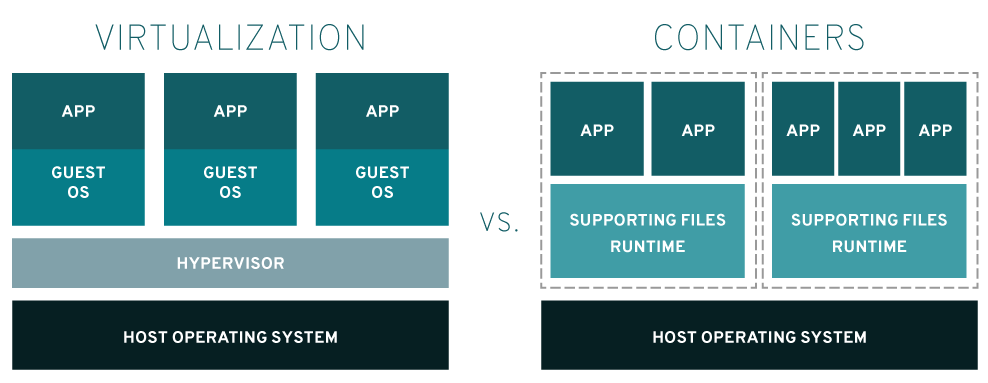
\includegraphics[width=0.8\textwidth]{img/virtualization-vs-containers.png}
    \caption{Virtualizzazione vs Containerizzazione\protect\footnotemark}
    \label{fig:virtualization-vs-containers}
\end{figure}
\FloatBarrier
\footnotetext{\url{https://www.redhat.com/en/blog/kubernetes-basics-sysadmins}}

\subsection{Implementazione dei container}

\subsubsection{Proprietà dei container}

L'approccio a container consente di ottenere le seguenti proprietà fondamentali:
\begin{itemize}
    \item \textbf{Isolamento} -- ogni container viene eseguito in una sandbox, cioè un ambiente virtualmente separato dall'host e dagli altri container. 
    \item \textbf{Consistenza} -- l'immagine del container è costruita ad hoc ed immutabile, quindi si ha la garanzia che l'esecuzione dell'applicazione al suo interno sia consistente.
    \item \textbf{Portabilità} -- un container può essere eseguito indipendentemente dall'infrastruttura sottostante e può essere quindi distribuito ovunque sia presente un Container Runtime.
\end{itemize}

\subsubsection{Container Image}
\label{subsec:oci}
La base di un container è la sua immagine, cioè un pacchetto auto-contenuto che include tutto il necessario per eseguire un'applicazione in modo coerente su qualsiasi ambiente che supporti la containerizzazione e segua lo standard aperto definito dall’OCI (Open Container Initiative).\\
Il file system dell'immagine è composto da diversi layer, che coincidono con le operazioni effettuate sullo stesso in fase di build dell'immagine stessa, che tipicamente avviene seguendo le indicazioni di manifest come il Dockerfile. Le immagini dei container possono essere memorizzate in dei Registry e versionate tramite tag; fra i container registry più diffusi troviamo Docker Hub, Quay.io e Google Container Registry.

\subsubsection{Container Runtime}

Il \texttt{Container Runtime} (abbreviato CR) è il componente che si occupa di istanziare le risorse richieste e dell'esecuzione del container\cite{Martin2018Exploring}. Uno dei compiti principali del CR è quello di isolare i processi e limitarne le risorse, per questo vengono utilizzati principalmente due strumenti messi a disposizione dal kernel Linux:
\begin{itemize}
    \item \texttt{Namespaces} -- utilizzati per isolare le risorse del sistema Linux, i principali sono:
    \begin{itemize}
        \item PID Namespace -- isola i processi del container.
        \item Network Namespace -- crea un'interfaccia di rete virtuale per il container.
        \item Mount Namespace -- fornisce un filesystem separato per il container.
        \item User Namespace -- permette l’esecuzione con utenti con privilegi ridotti.
    \end{itemize}

    \item \texttt{CGroups} -- utilizzati per limitare le risorse hardware come RAM, CPU, velocità di scrittura su disco ed accesso a dispositivi come GPU e periferiche.
    
\end{itemize}

Il CR si occupa inoltre di configurare il file system del container con strumenti come OverlayFS e di creare interfacce di rete virtuali esclusive al container.\\
Fra i Container Runtime troviamo containerd, CRI-O e Podman.

\subsection{Docker}

Docker è una piattaforma di containerizzazione\cite{Anderson2015Docker} che consente di creare, distribuire ed eseguire applicazioni all'interno di container.\\
Il componente principale del framework è il Docker Engine, un componente che integra il Container Runtime aggiungendo funzionalità per deployare e gestire più facilmente i container, fra i quali Docker Daemon, Docker CLI e Docker API. Il primo è il componente che si occupa della gestione dei container tramite il runtime (tipicamente containerd), mentre CLI ed API servono per comunicare con il servizio in background. Docker mette inoltre a disposizione delle risorse come volumi e network virtualizzate per facilitare il deploy delle applicazioni.\\

\subsubsection{Dockerfile}

Il dockerfile è diventato lo standard de facto per quanto riguarda la definizione di immagini per container; consiste in un file testuale nel quale vengono specificate tutte le istruzioni necessarie per la costruzione del container. Ogni istruzione che modifica il file system dell'immagine aggiunge un layer alla stessa, mentre le altre vengono interpretate dal demone di Docker per configurarla.
Di seguito viene riportato un esempio di un Dockerfile utilizzabile per eseguire uno script Python [\ref{code:dockerfile_example}].

\vspace{0.5cm}
\begin{lstlisting}[language=Dockerfile, caption={Esempio Dockerfile per script Python}, captionpos=b, label={code:dockerfile_example}]
    FROM python:3.11-slim
    
    LABEL maintainer="example@example.com"
    LABEL version="1.0"
    
    WORKDIR /app
    
    COPY requirements.txt .
    RUN pip install --no-cache-dir -r requirements.txt
    
    COPY . .
    
    ENV APP_ENV=production
    ENV PORT=5000
    
    EXPOSE 5000
    
    RUN groupadd -r appuser && useradd -r -g appuser appuser
    USER appuser
    
    ENTRYPOINT ["python"]
    CMD ["app.py"]
\end{lstlisting}

Fra le istruzioni riportate nel dockerfile analizziamo le più importanti:
\begin{itemize}
    \item \textbf{FROM} specifica l'immagine di base da cui Docker partirà la costruzione di quella nuova.
    \item \textbf{COPY} può essere utilizzata per copiare files o intere directory dal file system in cui sta eseguendo Docker dentro al container.
    \item \textbf{RUN} esegue dei comandi all'interno del container; tipicamente viene utilizzato per aggiornare le dipendenze utilizzate poi dall'applicazione.
    \item \textbf{ENV} imposta delle variabili d'ambiente all'interno del container.
    \item \textbf{EXPOSE} espone la porta specificata fuori dal container, in modo che sia raggiungibile dall'host in cui sta girando Docker.
    \item \textbf{ENTRYPOINT} e \textbf{CMD} vengono utilizzati per impostare il comando che partirà di default all'avvio del container (per esempio l'esecuzione dell'applicazione).
\end{itemize}

\subsubsection{Docker Compose}

Docker Compose è uno strumento che semplifica l’orchestrazione e la gestione di applicazioni composte da più container. Utilizza un file di configurazione in formato Yaml per definire  reti, variabili d'ambiente e volumi necessari all'esecuzione dell'applicazione.\\
All'interno del file \texttt{docker-compose.yaml} vengono descritti i servizi, che corrispondono a istanze di container, insieme alle policy da applicare a runtime:

\begin{lstlisting}[language=yaml, caption={Esempio docker-compose}, captionpos=b, label={code:dockercompose}]
    services:
      app:
        image: myapp:latest
        restart: always
        deploy:
          restart_policy:
            condition: on-failure
            delay: 5s
            max_attempts: 3
            window: 120s
        ports:
          - "8080:8080"
        environment:
          - APP_ENV=production
    
      db:
        image: postgres:15
        restart: unless-stopped
        deploy:
          restart_policy:
            condition: any
        environment:
          POSTGRES_USER: user
          POSTGRES_PASSWORD: password
        volumes:
          - db-data:/var/lib/postgresql/data
    
    volumes:
      db-data:
\end{lstlisting}

Nell'esempio mostrato dal Listing \ref{code:dockercompose} possiamo notare come siano presenti configurazioni simili a quelle del Dockerfile (come env e port) che andranno infatti ad aggiungersi o a sovrascrivere quelle specificate nell'immagine; le altre policy sono dedicate al deployment e alla gestione dei container a runtime (come la restart\_policy).\\
Docker Compose risulta uno strumento che semplifica notevolmente la gestione del lifecycle dei container e consente l'integrazione con tool di CI/CD e la simulazione di ambienti complessi indipendentemente dalla macchina in cui viene eseguito, facilitando così anche il lavoro dei developer che necessitano di  un'infrastruttura di testing a basso costo.

\subsection{Kubernetes}

Kubernetes è una piattaforma open-source per l'orchestrazione e la gestione di container. Automatizza il deployment, la scalabilità e la gestione delle applicazioni containerizzate.
L'architettura di Kubernetes\cite{kubernetesComponents} si basa su un modello \textbf{Master-Worker} distribuito\cite{Rejiba2022Custom}, con componenti che collaborano per gestire i container.

\subsubsection{Nodo Master (Control Plane)}
Il Control Plane è responsabile della gestione globale del cluster e include:
\begin{itemize}
    \item \textbf{API Server} -- punto di ingresso per tutte le richieste verso il cluster. Espone le API di Kubernetes e valida le richieste.
    \item \textbf{Scheduler} -- è il componente che si occupa del deployment dei container e dell'orchestrazione degli stessi nei vari nodi basandosi sulle metriche prodotte dal cluster (come RAM residua, utilizzo CPU e numero di Pod) o su policy specificate dall'utente (come i node\_selector).
    \item \textbf{etcd}: Database chiave-valore distribuito che memorizza le informazioni del cluster, inclusi i segreti, le configurazioni e i metadati. 
\end{itemize}

Il processo di deployment all'interno dei vari componenti segue tipicamente questo flusso:
\begin{enumerate}
    \item \textbf{API Server} riceve una richiesta, può essere una nuova configurazione, una modifica di una già esistente o la rimozione di una risorsa.
    \item API Server inserisce la nuova configurazione in \textbf{etcd}, aggiornando tutte le istanze distribuite nei vari nodi Master.
    \item lo \textbf{Scheduler} controlla ripetutamente lo stato di etcd in attesa di modifiche. Una volta rilevata una modifica si occupano di applicarla nei vari nodi.
\end{enumerate}

Questa suddivisione architetturale facilita la scalabilità e la distribuzione del cluster: l'unico componente stateful infatti è \texttt{etcd}, quindi una volta messo questo ``in sicurezza" è posssibile ripristinare il cluster indipendente dagli altri componenti. Essendo un database distribuito implementa meccanismi di elezione e quorum sui dati, motivo per il quale il numero dei master deve essere sempre dispari (1, non consigliato, 3, 5 etc.). Finché saranno presenti \(\frac{n\_nodi\_etcd}{2} + 1\) istanze di etcd attive ed healthy, il cluster continuerà a funzionare correttamente.

\subsubsection{Nodo Worker}
I nodi Worker eseguono le applicazioni containerizzate che non fanno parte di quelle del sistema Kubernetes; sono i nodi che di fatto eseguono i servizi deployati dall'utente e sono composti da due componenti principali:
\begin{itemize}
\item \textbf{Kubelet} -- agente che comunica con i Master per ricevere istruzioni sul deployment delle risorse e per comunicare le metriche del nodo.
\item \textbf{Kube Proxy} -- gestisce il bilanciamento del carico e le regole di rete dei servizi esposti sul nodo.
\end{itemize}

\subsubsection{Container Runtime}

Kubernetes utilizza l'interfaccia \texttt{Container Runtime Interface (CRI)} per comunicare con il CR sottostante, consentendo la compatibilità con diversi tipi di runtime come CRI-O (attualmente utilizzato di default) o containerd.\\

Riassumendo, la struttura completa di Kubernetes può essere schematizzata come nella seguente Figura \ref{fig:kube_arch}.
\FloatBarrier
\begin{figure}[h]
    \centering
    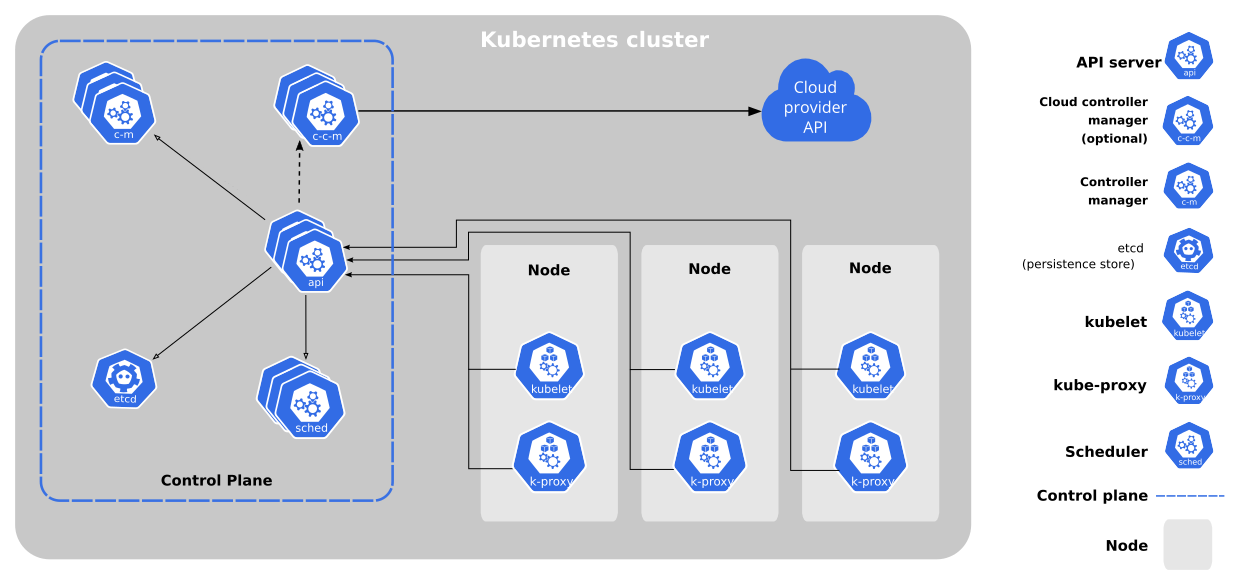
\includegraphics[width=\textwidth]{img/components-of-kubernetes.png}
    \caption{Architettura di Kubernetes \protect\footnotemark}
    \label{fig:kube_arch}
\end{figure}
\FloatBarrier
\footnotetext{\url{https://kubernetes.io/docs/concepts/overview/components/}}

\subsubsection{Deploy applicazioni su Kubernetes}

Ogni risorsa di Kubernetes può essere descritta tramite un manifest yaml con un approccio simile a quello di Docker Compose, la differenza è che su Kubernetes sono presenti molti più oggetti che soddisfano necessità specifiche in modo più ottimizzato e configurabile.\\
Ogni elemento di Kubernetes è associato al proprio \textbf{Namespace}, una suddivisione logica utilizzata per gestire e isolare le risorse all'interno di un cluster. Permette di organizzare e gestire gruppi di risorse in modo indipendente, migliorando la scalabilità e la sicurezza di ambienti complessi.

\subsubsection{Oggetti per il deployment di risorse}

 L'unità minima di esecuzione all'interno del cluster è il \textbf{Pod}, un'istanza di applicazione in esecuzione che può contenere uno o più container che condividono lo stesso spazio di rete e di storage. I Pod hanno un ciclo di vita definito e vengono creati, programmati ed eseguiti su uno specifico nodo. Ogni Pod è associato a una serie di risorse come le richieste e i limiti di CPU e di memoria, e può essere configurato con volumi persistenti per la gestione dello storage; possono inoltre comunicare tra loro tramite indirizzi IP univoci e supportano la configurazione di probe di readiness e liveness per il monitoraggio dello stato di salute.
 
I Pod non vengono generati direttamente dall'utente, bensì da altre risorse dedicate. Quella principalmente utilizzata per il deploy di applicazioni stateless è il \textbf{Deployment} e consente di:
\begin{itemize}
    \item Gestire il ciclo di vita dei Pod e il monitoraggio degli stessi. 
    \item Definire probe di readiness e liveness per controllare lo stato di salute delle applicazioni e impedire l'invio di traffico ai Pod non pronti.
    \item Specificare strategie di aggiornamento dei Pod, come RollingUpdate e Recreate.
    
\end{itemize}

Kubernetes offre anche diversi componenti per gestire applicazioni con esigenze specifiche. Lo \texttt{StatefulSet} è pensato per applicazioni stateful, garantisce un ordine controllato al deployment e fornisce volumi dedicati ai Pod. Il \texttt{DaemonSet}, invece, assicura che determinati Pod vengano eseguiti su ogni nodo, risultando utile per servizi infrastrutturali come il monitoraggio e il logging. Per l'esecuzione di processi batch e operazioni pianificate, Kubernetes mette a disposizione il \texttt{Job}, che assicura il completamento di un'attività, e il \texttt{CronJob}, che ne consente l'esecuzione ricorrente seguendo una pianificazione definita.

\subsubsection{Oggetti per la configurazione dei Pod}

Kubernetes mette a disposizione due oggetti per la configurazione dinamica dei Pod:

\begin{itemize}
    \item La \textbf{ConfigMap}, una risorsa utilizzata per memorizzare informazioni di configurazione non sensibili sotto forma di coppie chiave-valore. Permette di separare la configurazione dal codice dell'applicazione, facilitando la gestione e l'aggiornamento delle impostazioni senza dover ricreare i container.
    \item I \textbf{Secret} servono per memorizzare dati sensibili come password, chiavi API o certificati. A differenza delle ConfigMap, i Secret sono codificati in base64 e vengono archiviati in modo più sicuro.
\end{itemize}

Sia Secret che ConfigMap possono essere acceduti ai Pod tramite variabili d'ambiente e/o file montati come volumi all'interno dei container.

\subsubsection{Persistenza dei Pod}

I Volumi permettono di gestire la persistenza dei dati tra i cicli di vita dei container. Ogni Pod può avere uno o più volumi montati, condivisi tra i container dello stesso Pod. Vengono gestiti tramite due risorse:
\begin{itemize}
    \item il \textbf{PersistentVolume} rappresenta una porzione di storage fisico o di rete fornito dal cluster in base alla classe del PV, cioè un'interfaccia utilizzata per integrare sistemi di storage diversi (come LocalStorage, NFS, CephFS etc) e standardizzarne le operazioni.
    \item Il \textbf{PersistentVolumeClaim} è una richiesta di storage da parte di un Pod. I Pod non interagiscono direttamente con i PersistentVolume, ma ne richiedono una porzione tramite i PVC.
\end{itemize}
Questo approccio disaccoppia ulteriormente il runtime dalla infrastruttura sottostante.

\subsubsection{Oggetti per il networking}

La risorsa principale utilizzata per il networking interno a Kubernetes è il Service. Esso fornisce un'astrazione di rete stabile per esporre uno o più Pod come un unico endpoint. Poiché i Pod sono dinamici e possono essere creati o distrutti, il Service garantisce che l'applicazione rimanga accessibile senza dover conoscere i singoli indirizzi IP; la selezione dei Pod avviene tramite un PodSelector basato su labels.\\
La creazione di un Service porta a tre funzionalità principali:
\begin{itemize}
    \item Indirizzo IP Virtuale (\texttt{ClusterIP}): fornisce un endpoint virtuale statico per l'applicazione.
    \item Bilanciamento del carico: distribuisce il traffico tra più Pod in base alla policy specificata.
    \item Risoluzione dei nomi: assegna un nome DNS stabile ai Pod.
\end{itemize}

Un'altra risorsa molto importante è l'\textbf{Ingress}, che si occupa di esporre un Service al di fuori del cluster Kubernetes ed assegnarlo ad uno o più record DNS, utilizzati poi dall'IngressController (un reverse proxy) per identificare il servizio target delle richieste ricevute dai Kube Proxy del cluster.

\subsubsection{Kubernetes nel Cloud Computing}

Grazie al suo approccio alle applicazioni containerizzate, unito alla scalabilità e portabilità della sua infrastruttura, Kubernetes è diventato uno degli strumenti di riferimento nel panorama del Cloud Computing.
Queste caratteristiche lo rendono anche un candidato ideale per l'adozione del modello Fog Computing, dove le applicazioni devono essere eseguite sia in ambienti Cloud che su nodi Edge, dovendo garantire tempi di migrazione ridotti, scalabilità semplice e un bilanciamento efficace dei carichi di lavoro.\\
Nonostante i suoi punti di forza, la complessità architetturale di Kubernetes può incontrare colli di bottiglia nelle prestazioni, come la latenza nella distribuzione dei dati e un bilanciamento del carico inefficiente. La ricerca si è concentrata sull'ottimizzazione di Kubernetes per migliorare il recupero da disastri, l'autoscaling e le strategie di pianificazione, portando a significativi miglioramenti delle prestazioni, come una riduzione dell'uso della CPU e della memoria e tassi di fallimento delle richieste più bassi\cite{Mondal2024On}.



\section{WebAssembly}
\label{sec:webassembly}

WebAssembly\cite{WasmSpec24} (Wasm) è una tecnologia emersa negli ultimi dieci anni in seguito alla diffusione delle applicazioni web e alla necessità di trovare un modo performante per eseguire codice sui browser.\\
Le applicazioni web infatti usano Javascript, un linguaggio interpretato molto comodo per definire logiche legate al frontend ma altrettanto carente in termini di performance.\\
La soluzione proposta da WebAssembly è quella di un programma precompilato interpretabile dal browser ed integrabile all'interno del codice Javascript; questo permette di programmare i task computazionalmente onerosi in linguaggi più adatti (come C, C++, Rust e Go) e precompilare il codice in un formato portabile e performante.\\
WebAssembly infatti è un bytecode, cioè un linguaggio intermedio più astratto tra il linguaggio macchina e il linguaggio di programmazione, progettato per essere eseguito da Runtime che ottengono performance simili a quelle native (o superiori nel caso di linguaggi interpretati come Javascript e Python).\\
Questo modello consente di sviluppare applicazioni senza preoccuparsi dell'architettura dell'infrastruttura sottostante: lo stesso codice WebAssembly può essere eseguito su RISC-V, x86, ARM o qualsiasi altra architettura, dato che è sufficiente che il Runtime sia stato implementato per la stessa; questo approccio è simile a quello adottato da Java con i suoi programmi precompilati (come il bytecode) ed eseguiti sulla Java Virtual Machine.

\subsection{Wasm Runtime}

I runtime di WebAssembly sono ambienti software che possono eseguire i file binari Wasm. Questi runtime possono essere implementati in vari modi, ad esempio all'interno dei browser, e fornire un ambiente di esecuzione per il codice Wasm, con funzionalità come gestione della memoria, sicurezza e ottimizzazione delle prestazioni.\\
Infatti Wasm, in modo analogo ai container, viene eseguito all'interno di una sandbox e non può accedere direttamente alle risorse della macchina. L'unico modo per comunicare con un modulo Wasm è tramite delle interfacce implementate da funzioni sul codice e invocabili da ambienti esterni.\\
La leggerezza di Wasm si adatta perfettamente ai sistemi embedded, dove la dimensione del codice e le prestazioni sono fattori critici. I runtime Wasm embedded sono tipicamente utilizzati per dispositivi IoT, microcontrollori e altre applicazioni che richiedono un basso overhead di memoria e un'esecuzione efficiente. Ad esempio, il Wasm Micro Runtime (WAMR)\cite{bytecodealliance_wasm_micro_runtime} è un popolare runtime embedded per Wasm, progettato per essere altamente ottimizzato per i sistemi embedded, con una dimensione binaria ridotta e un basso overhead di memoria. Altri runtime diffusi sono Wasmtime\cite{wasmtime_introduction} e Wasmedge\cite{wasmedge_wasmedge}.\\
La maggior parte dei runtime supporta due tipi di compilazione di codice Wasm, cioè quella JIT (Just in time) utilizzata principalmente dai browser, oppure quella AOT (Ahead of time) che consiste nel precompilare il codice in un pacchetto .wasm e fornirlo direttamente al runtime, come nell'esempio riportato nella Figura seguente \ref{fig:wasm_workflow}.

\FloatBarrier
\begin{figure}[h]
    \centering
    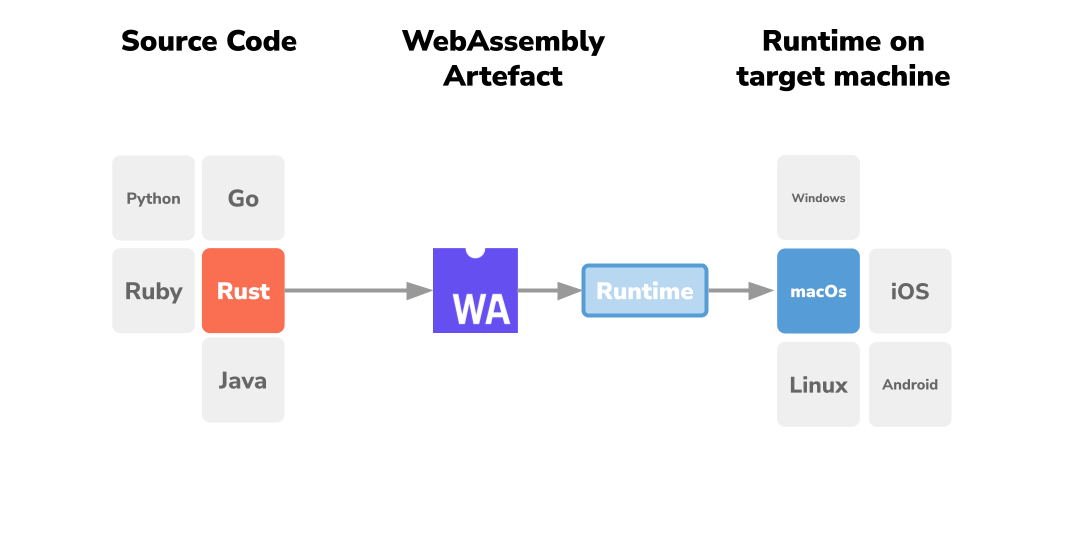
\includegraphics[width=0.9\textwidth]{img/wasm-runtime.png}
    \caption{Wasm workflow\protect\footnotemark}
    \label{fig:wasm_workflow}
\end{figure}
\FloatBarrier
\footnotetext{\url{https://b-nova.com/en/home/content/how-containerless-works-thanks-to-web-assembly-runtimes/}}

\subsubsection{Wasm Compilers}

Esistono diverse infrastrutture di compilazione che possono essere utilizzate per compilare codice in WebAssembly, tra cui \textbf{LLVM} (Low-Level Virtual Machine), una delle infrastrutture di compilazione open-source più diffuse. Grazie al supporto di LLVM molti tool riescono a generare codice in formato WebAssembly, fra cui notiamo:
\begin{itemize}
    \item \texttt{Emscripten}\cite{Jiang2017Quick}, una toolchain che consente di compilare codice scritto in C/C++ e altri linguaggi supportati.
    \item \texttt{TinyGo}\cite{Plauska2022Performance}, che garantisce un forte supporto alla tecnologia Wasm per il linguaggio Golang.
\end{itemize}
Inoltre, il linguaggio di programmazione Rust integra un proprio backend Wasm, semplificando la compilazione diretta del codice Rust in WebAssembly.


\subsection{Specifica moduli Wasm}

Un modulo Wasm è l'unità fondamentale di codice eseguibile in WebAssembly e rappresenta un file binario (con estensione .wasm) che contiene istruzioni, dati e metadati compilati da linguaggi di alto livello. Ogni modulo è suddiviso internamente in sezioni, ognuna con uno scopo specifico:
\begin{itemize}
    \item \textbf{Definizioni e Tipi di Dati}
    \begin{itemize}
        \item \texttt{Type} -- definisce la firma delle funzioni (parametri e tipo di ritorno).
        \item \texttt{Global} -- variabili globali utilizzabili dalle funzioni.
    \end{itemize}
    
    \item \textbf{Gestione della Memoria e Tabelle}
    \begin{itemize}
        \item \texttt{Memory} -- definisce la memoria lineare utilizzata dal modulo.
        \item \texttt{Table} -- gestisce funzioni indirette tramite tabelle di riferimento.
        \item \texttt{Data} -- inizializza i dati nella memoria lineare.
    \end{itemize}
    
    \item \textbf{Interoperabilità e Interfacce Esterne}
    \begin{itemize}
        \item \texttt{Import} -- risorse esterne richieste dal modulo (funzioni, memoria, variabili).
        \item \texttt{Export} -- funzioni o variabili rese disponibili all'esterno.
    \end{itemize}
    
    \item \textbf{Codice e Funzioni}
    \begin{itemize}
        \item \texttt{Function} -- elenca le funzioni definite nel modulo.
        \item \texttt{Code} -- contiene le istruzioni Wasm associate alle funzioni.
    \end{itemize}
\end{itemize}

Grazie a questa specifica WebAssembly è in grado di eseguire codice indipendentemente dal linguaggio in cui è stato scritto in origine. Questa specifica risulta però complicata da utilizzare per sviluppatori non esperti in Wasm, inoltre è molto difficile far comunicare moduli Wasm differenti in modo dinamico.

\subsection{Componenti Wasm e specifica WASI}

\subsubsection{Wasm Components}
\label{sec:wasm_components}

Per risolvere le problematiche riportate nel paragrafo precedente la specifica Wasm è stata estesa aggiungendo un nuovo modello di esecuzione, cioè il componente. Un componente WebAssembly\cite{webassembly_component_model} è un'estensione del modulo standard, introdotta per migliorare la modularità, la composizione e l'interoperabilità tra diversi moduli e linguaggi di programmazione.\\
A differenza di un modulo standard, che rappresenta un'unità eseguibile isolata, un componente WebAssembly consente di combinare più moduli in modo dinamico, facilitando l'integrazione di codice eterogeneo e il riutilizzo delle funzionalità.

\subsubsection{WIT}

I componenti sono implementati come wrapper di uno o più moduli WebAssembly e utilizzano un linguaggio chiamato \texttt{WIT (Wasm Interface Type)}, tramite il quale è possibile definire ``contratti" e specificare le interfacce in modo più intuitivo.\\
WIT aggiunge definizioni per tipi primitivi e complessi, introduce il tipo di ritorno di funzione opzionale e il supporto a definizioni in più file.

\begin{itemize}
    \item \textbf{Tipi Primitivi}
    \begin{itemize}
        \item \texttt{bool} -- valore booleano (vero o falso).
        \item \texttt{u8} -- intero senza segno a 8 bit.
        \item \texttt{s32} -- intero con segno a 32 bit.
        \item \texttt{s64} -- intero con segno a 64 bit.
        \item \texttt{float32} -- numero a virgola mobile a 32 bit.
        \item \texttt{float64} -- numero a virgola mobile a 64 bit.
    \end{itemize}

    \item \textbf{Tipi Complessi}
    \begin{itemize}
        \item \texttt{string} -- sequenza di caratteri UTF-8.
        \item \texttt{list<T>} -- lista omogenea di elementi di tipo \texttt{T}.
        \item \texttt{record} -- struttura con campi nominati.
        \item \texttt{variant} -- tipo di unione (enumerazioni con payload opzionali).
        \item \texttt{tuple} -- gruppo ordinato di tipi eterogenei.
    \end{itemize}

    \item \textbf{Tipi di Risultato}
    \begin{itemize}
        \item \texttt{option<T>} -- valore opzionale (simile a \texttt{Option} in Rust).
        \item \texttt{result<T, E>} -- risultato di successo o errore (simile a \texttt{Result} in Rust).
    \end{itemize}

    \item \textbf{Tipi di Composizione}
    \begin{itemize}
        \item \texttt{import} -- permette di importare funzioni o tipi da altri moduli.
        \item \texttt{export} -- esporta funzioni o tipi per essere utilizzati da altri componenti.
    \end{itemize}
\end{itemize}

L'enorme vantaggio di questo approccio è che introduce la possibilità di utilizzare dei moduli Wasm precompilati come librerie, aumentando notevolmente la modularità e la semplicità di utilizzo anche per sviluppatori meno esperti. Ecco un esempio di un semplice file WIT \ref{code:wit} che esporta due funzioni implementate nel codice:
\begin{lstlisting}[language=yaml, caption={Esempio file WIT}, captionpos=b, label={code:wit}]
    package default:math;
    
    interface math {
        add: func(a: s32, b: s32) -> s32
        multiply: func(a: s32, b: s32) -> s32
    }
\end{lstlisting}

\subsubsection{WASI}
\label{sec:wasi}
\texttt{WebAssembly System Interface (WASI)}\cite{WASI2024} è uno standard che specifica un'interfaccia simile a POSIX progettata per consentire ai moduli Wasm di interagire in modo sicuro ed efficiente con il sistema operativo e le risorse di sistema, come file system, rete e orologio di sistema.\\
Nel momento in cui viene scritto questo elaborato la versione stabile di WASI è la \texttt{Preview 0.2}\cite{WASI2024}, basata sul modello a componenti e supportata principalmente dai compilatori di Rust e Go (in particolare Tinygo). Le interfacce API attualmente disponibili sono elencate nella tabella \ref{tab:wasi_interfaces}.

\begin{table}[h]
    \centering
    \small
    \begin{tabular}{|l|l|}
        \hline
        \textbf{Interfaccia} & \textbf{Repository} \\
        \hline
        \arrayrulecolor[gray]{0.7}
        \arrayrulewidth=0.4pt
        Clocks     & \url{https://github.com/WebAssembly/wasi-clocks} \\
        \hline
        Random     & \url{https://github.com/WebAssembly/wasi-random} \\
        \hline
        Filesystem & \url{https://github.com/WebAssembly/wasi-filesystem} \\
        \hline
        Sockets    & \url{https://github.com/WebAssembly/wasi-sockets} \\
        \hline
        CLI        & \url{https://github.com/WebAssembly/wasi-cli} \\
        \hline
        HTTP       & \url{https://github.com/WebAssembly/wasi-http} \\
        \hline
    \end{tabular}
    \caption{Interfacce WASI Preview 0.2 e relativi repository}
    \label{tab:wasi_interfaces}
\end{table}

Inoltre, WASI adotta il modello di sicurezza basato su capability\cite{Sangeeta23} (capability-based security), in cui il runtime WebAssembly deve concedere esplicitamente l'accesso a ciascuna risorsa (come socket o file), creando così un ambiente di esecuzione sandboxed e sicuro.\\

\subsubsection{wRPC}
\label{sec:wrpc}

Un'implementazione interessante dell'ecosistema Wasm + WASI è il progetto \texttt{wRPC}\cite{bytecodealliance_wrpc}(WIT-over-RPC), un framework RPC sviluppato dalla Bytecode Alliance (l'organizzazione che si occupa di sviluppare e mantenere le tecnologie legate a Wasm come WASI\cite{WASI2024} e runwasi\cite{containerd_runwasi} di conteinerd).\\
wRPC è un protocollo progettato per facilitare l'esecuzione di funzionalità definite in WIT su reti o altri mezzi di comunicazione. Le sue principali applicazioni includono:
\begin{itemize}
    \item Plugin runtime Wasm esterni
    \item Comunicazione distribuita tra componenti Wasm
\end{itemize}
Sebbene wRPC sia stato progettato principalmente per i componenti Wasm, è completamente utilizzabile anche al di fuori del contesto Wasm, servendo come framework RPC generico. Utilizza la codifica della definizione del valore del modello dei componenti durante la trasmissione e supporta sia casi d'uso dinamici (basati, ad esempio, sull'introspezione del tipo di componente Wasm a runtime) che statici. Per i casi d'uso statici, wRPC fornisce generatori di binding WIT per i linguaggi Rust e Go.\\

\subsection{Wasm e tecnologie Cloud-Native}

In seguito agli sviluppi degli ultimi anni e all'implementazione di WASI e del modello a componenti, la tecnologia WebAssembly ha recentemente compiuto un'ulteriore evoluzione, cioè l'implementazione della specifica OCI [\ref{subsec:oci}].\\

\subsubsection{Wasm e Kubernetes}

Grazie a ciò, i Runtime WebAssembly possono essere utilizzati in maniera analoga ai diffusi Container Runtime e strumenti di orchestrazione come Kubernetes sono in grado di orchestrare componenti Wasm con comodità e vantaggi analoghi a quelli dei container standard\cite{10682874}.\\
L'integrazione fra Wasm e Kubernetes\cite{9978884} o tecnologie simili apre le porte a scenari fino ad ora impossibili o molto difficili da immaginare, come la possibilità di avere cluster Kubernetes distribuiti su nodi dalle architetture differenti (per esempio estendere un cluster AMD64 con un nodo RISC-V). \\
Infatti, utilizzando l'approccio a container standard sarebbe stato necessario generare un'immagine compatibile per ogni singola architettura, dato che il container condivide il kernel con l'host sottostante ed esso varia in base ad essa. Utilizzando Wasm invece questo problema viene risolto alla radice, in quanto lo stesso componente può essere eseguito indipendentemente dall'architettura sottostante: i problemi di compatibilità saranno infatti gestiti del Runtime e della specifica WASI.\\

\subsubsection{Wasm nel panorama dell'Edge-Cloud Continuum}

Nel contesto del Cloud ed Edge Computing\cite{Wallentowitz2022}, Wasm si sta affermando come una tecnologia fondamentale per lo sviluppo e l'esecuzione di applicazioni distribuite. La sua capacità di avviarsi in tempi brevissimi e di operare con un basso impatto sulle risorse lo rende ideale per implementare microservizi e funzioni serverless direttamente sui nodi periferici della rete, riducendo significativamente la latenza e migliorando la reattività delle applicazioni critiche.\\
Inoltre, Wasm facilita l'integrazione di componenti scritti in linguaggi differenti, promuovendo una composizione modulare delle applicazioni. Tale interoperabilità permette agli sviluppatori di aggiornare e scalare le soluzioni in maniera flessibile, sfruttando al contempo l'efficienza del modello esecutivo di Wasm. Un ulteriore vantaggio è rappresentato dalla possibilità di eseguire modelli di Machine Learning direttamente all'Edge, abilitando inferenze rapide e una gestione più sicura dei dati.\\
In conclusione, l'adozione di Wasm offre un nuovo paradigma per lo sviluppo di soluzioni performanti, sicure e scalabili, rispondendo efficacemente alle esigenze di un ecosistema sempre più dinamico e distribuito in dispositivi eterogenei e con architetture differenti, come mostrato nella Figura \ref{fig:wasm_devices}.

\FloatBarrier
\begin{figure}[h]
    \centering
    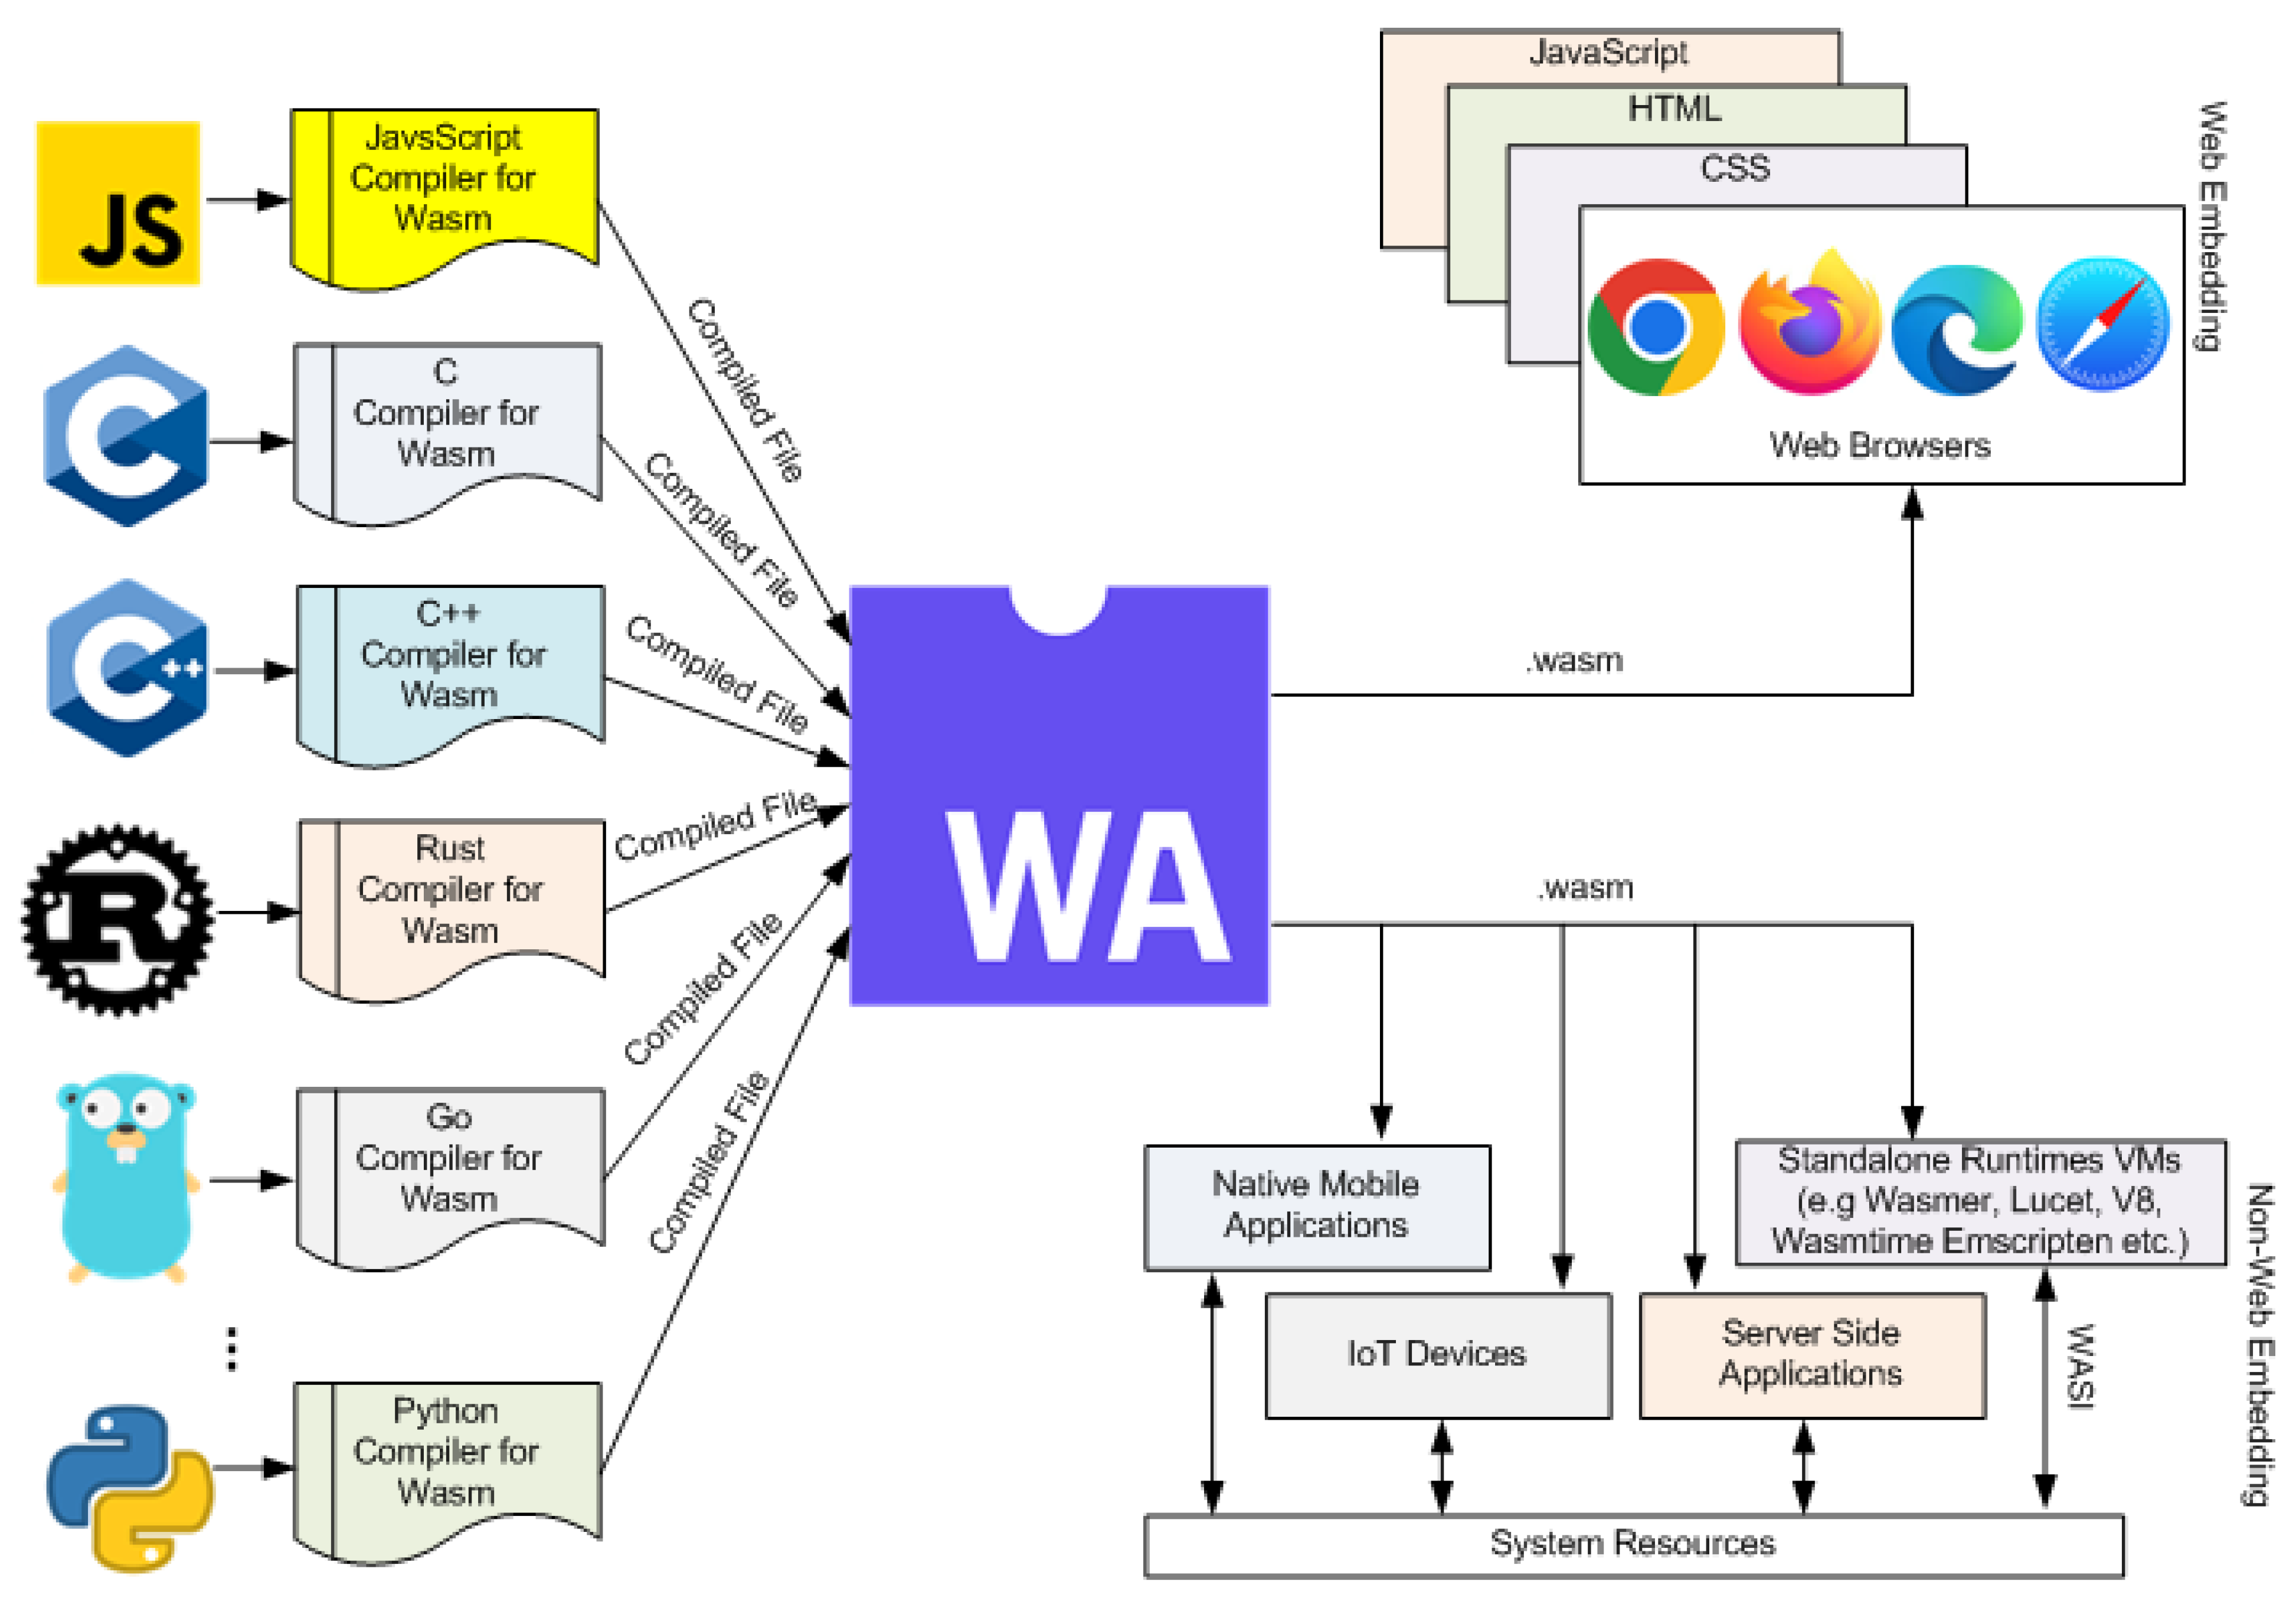
\includegraphics[width=0.85\textwidth]{img/wasm-distribution.png}
    \caption{Distribuzione codice WebAssembly\protect\footnotemark}
    \label{fig:wasm_devices}
\end{figure}
\FloatBarrier
\footnotetext{\small\url{https://www.researchgate.net/figure/WebAssembly-data-flow-architecture_fig1_373229823}}

\subsection{Framework e runtime distribuiti}

Da quando la tecnologia Wasm ha implementato la specifica OCI, sono nati molti framework che aiutano a gestire l'integrazione fra il mondo containerizzato e Wasm, in particolare vengono riportate le seguenti soluzioni:
\begin{itemize}
    \item \texttt{containerd} ha introdotto il supporto nativo a Wasm tramite il runtime WasmEdge\cite{containerd_runwasi} (per ora nella release beta). Grazie a ciò è possibile incorporare dei moduli Wasm all'interno di container utilizzando un semplice Dockerfile, come mostrato nel Listing \ref{code:dockerfile_example_wasm}.

    \item \texttt{Spinkube}\cite{spinkube_overview} è un framework open-source che consente di deployare dei moduli Wasm come Pod di Kubernetes tramite l'utilizzo di Custom Resource Definition e un Operator.
    
    \item \texttt{wasmCloud} è un altro framework simile a Spinkube, che però può essere utilizzato anche fuori dall'ambiente Kubernetes. 
\end{itemize}

\begin{lstlisting}[language=Dockerfile, caption={Esempio Dockerfile per modulo Wasm}, captionpos=b, label={code:dockerfile_example_wasm}]
    FROM scratch
    
    COPY ./main.wasm /main.wasm
    
    CMD ["serve","./main.wasm"]
\end{lstlisting}

\subsection{wasmCloud}
\label{sec:wasmcloud}

Verrà adesso approfondita questa soluzione, in quanto è quella che è stata utilizzata come base per questo progetto. wasmCloud\cite{wasmcloud} è una piattaforma per l'esecuzione di componenti WebAssembly distribuiti su diverse infrastrutture, dal Cloud all'Edge. Al centro della sua architettura c'è il \texttt{Lattice}, una rete mesh autoformante basata su \texttt{NATS}, che fornisce comunicazione affidabile e distribuita tra i vari nodi dell'applicazione. Ogni nodo esegue il \texttt{wasmCloud Host}, un runtime che gestisce l'esecuzione dei componenti WebAssembly e il collegamento dinamico con i provider esterni, come servizi di storage o HTTP.\\
La piattaforma si basa su contratti di interfaccia che definiscono le funzionalità richieste dai componenti, mentre i \texttt{Provider} forniscono implementazioni concrete di queste funzionalità, separando così la logica applicativa dall'infrastruttura. Per orchestrare e gestire le applicazioni in modo dichiarativo, wasmCloud utilizza \texttt{wadm} (WasmCloud Application Deployment Manager), che permette di definire e distribuire le topologie applicative senza configurare manualmente le connessioni.\\
Questa architettura consente di costruire applicazioni scalabili, portabili e sicure, riducendo al minimo la complessità di gestione dell'infrastruttura.\\
Approfondiamo adesso l'architettura di wasmCloud, partendo da NATS.

\subsubsection{NATS}

NATS è un sistema di messaggistica open-source ad alte prestazioni progettato per supportare applicazioni distribuite, architetture a microservizi, applicazioni IoT e sistemi Cloud-Native. Funziona come un middleware orientato ai messaggi, facilitando lo scambio di dati tra servizi e applicazioni attraverso un modello di comunicazione publish-subscribe.\\
L'architettura di NATS è modulare e può supportare le seguenti modalità di utilizzo:
\begin{itemize}
    \item Server standalone: un singolo server NATS. Può gestire milioni di messaggi al secondo, offrendo un'infrastruttura efficiente per la comunicazione tra client.

    \item Cluster: più server NATS possono essere raggruppati in un cluster per migliorare la tolleranza ai guasti e la scalabilità. I server all'interno di un cluster comunicano tra loro per garantire la distribuzione e la disponibilità dei messaggi.

    \item Super-Cluster: quando è necessaria una scalabilità ancora maggiore, più cluster possono essere collegati insieme per formare un supercluster. Essi utilizzano connessioni gateway per instradare i messaggi tra cluster diversi, ottimizzando il traffico e migliorando la resilienza del sistema e garantire una geodistribuzione del servizio (Figura \ref{fig:nats_supercluster}).

    \item Leaf Node: un singolo server NATS che si estende da un cluster o da un server remoto. I Leaf node sono ideali per scenari come Edge computing o data center che necessitano di essere collegati a una distribuzione NATS più ampia, permettendo di collegare in modo trasparente ambienti on-premise e Cloud (Figura \ref{fig:nats_leaf}). Inoltre un nodo Leaf può continuare ad instradare pacchetti localmente anche se perde la connessione con il server/cluster remoto, permettendo alle applicazioni situate sull'Edge di funzionare anche in casi di connettività scadente.
\end{itemize}

\FloatBarrier
\begin{figure}[h]
    \centering
    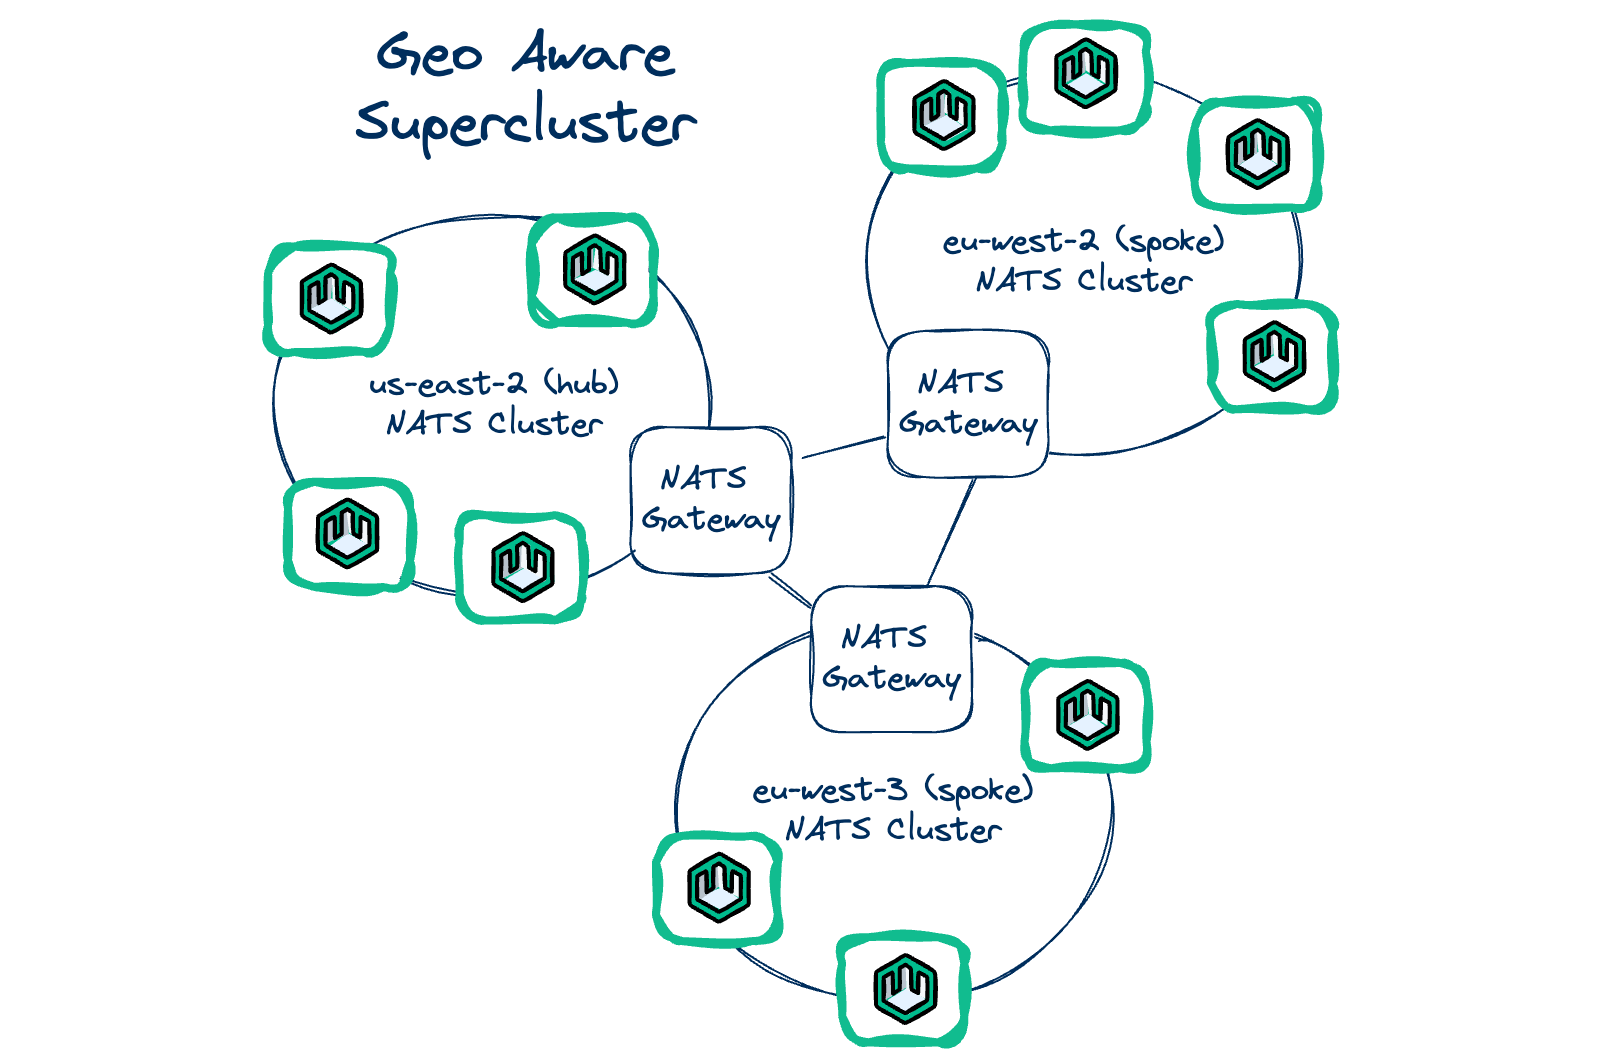
\includegraphics[width=0.9\textwidth]{img/nats-supercluster.png}
    \caption{Supercluster NATS geodistribuito\protect\footnotemark}
    \label{fig:nats_supercluster}
\end{figure}
\FloatBarrier

\footnotetext{\url{https://wasmcloud.com/docs/ecosystem/nats/}}

\FloatBarrier
\begin{figure}[ht]
    \centering
    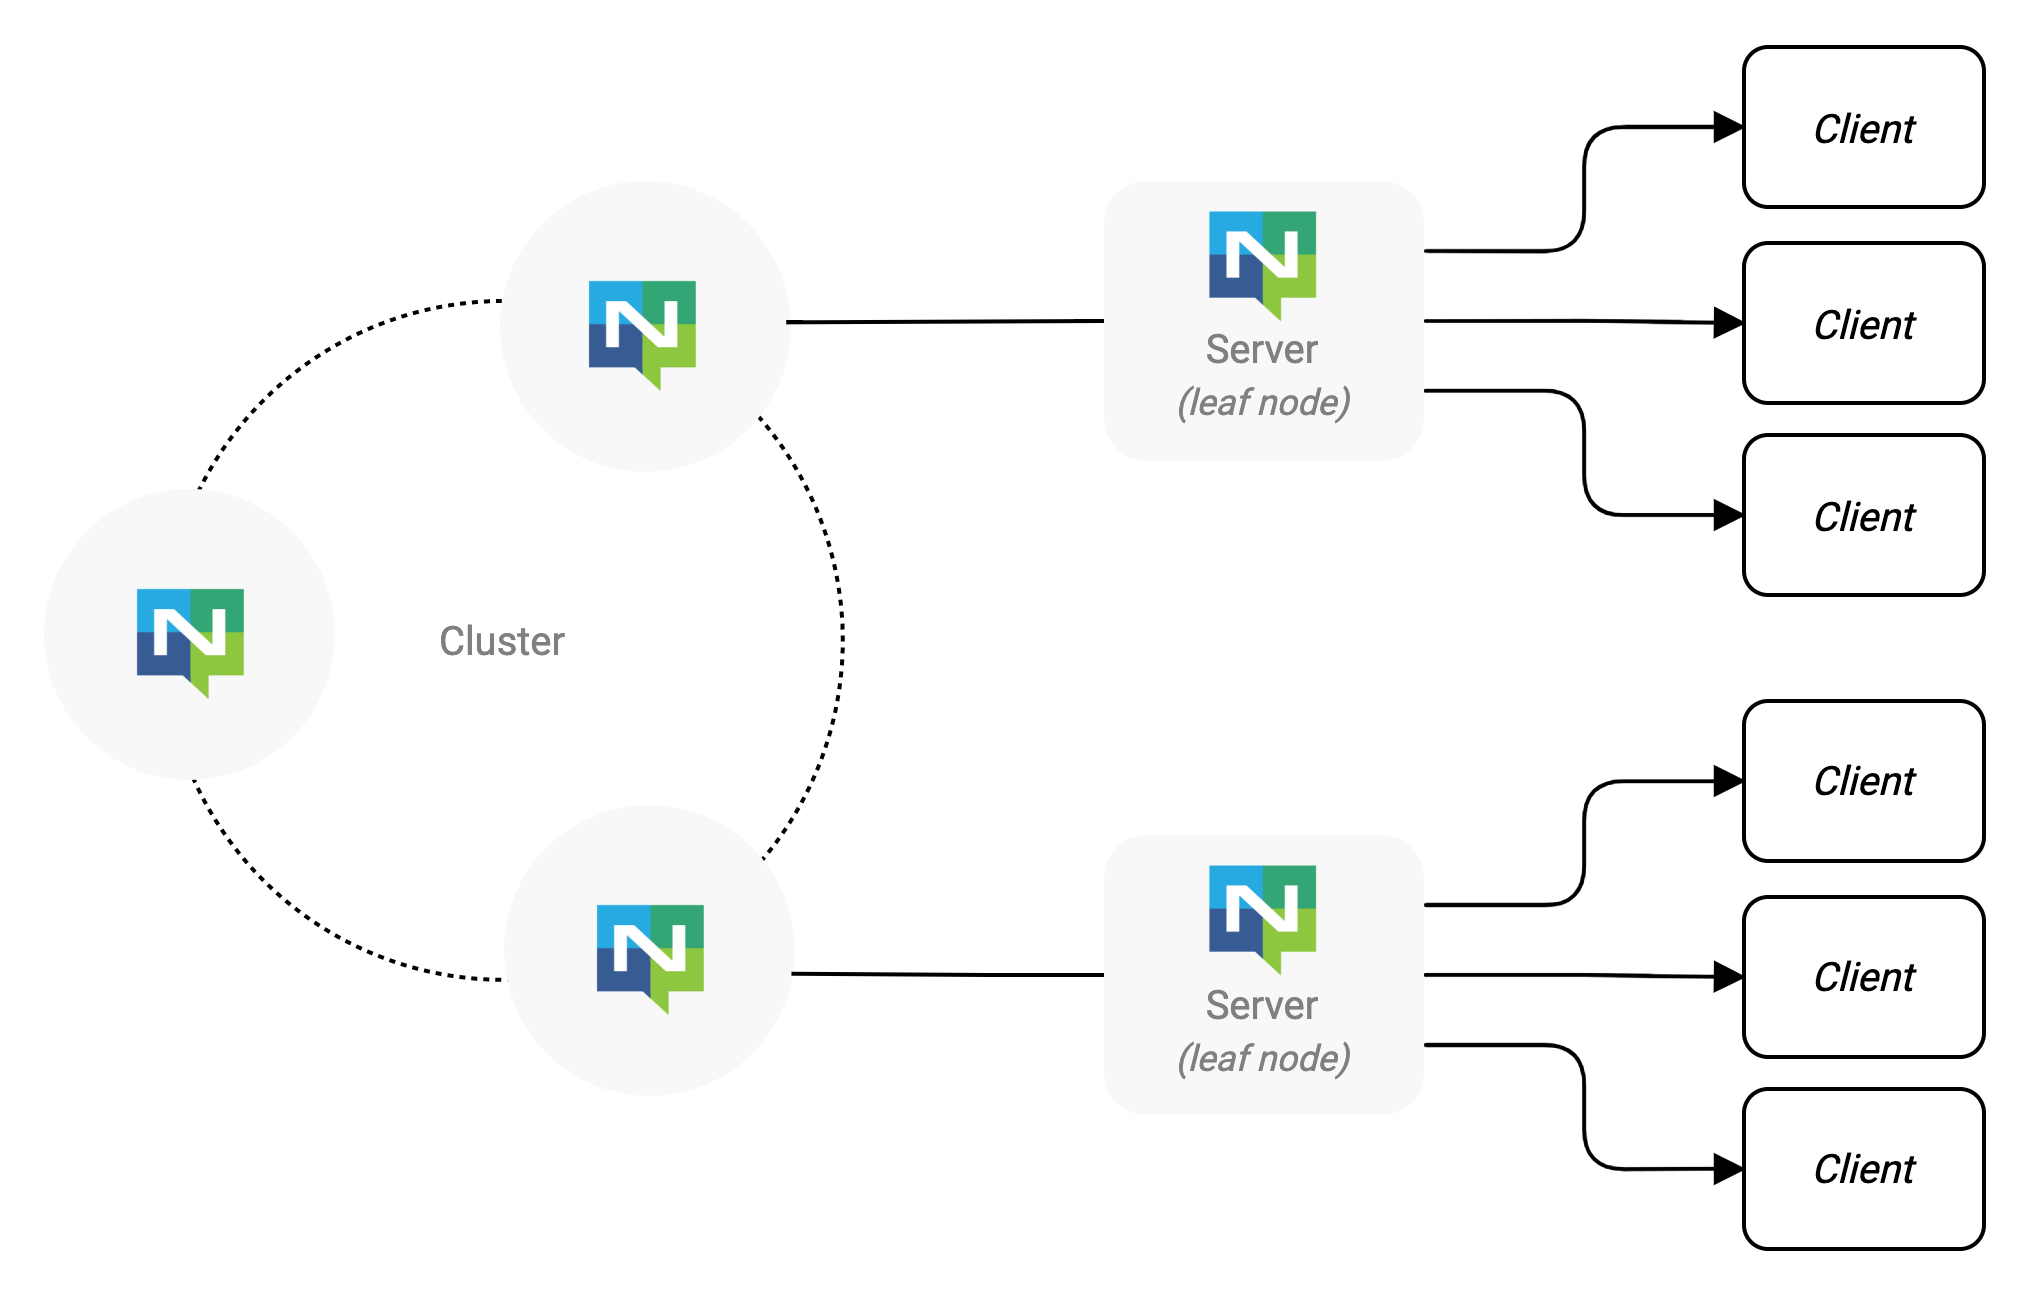
\includegraphics[width=0.8\textwidth]{img/nats-leaf.png}
    \caption{Cluster NATS con nodi Leaf\protect\footnotemark}
    \label{fig:nats_leaf}
\end{figure}
\FloatBarrier

\footnotetext{\url{https://www.karanpratapsingh.com/blog/nats-topology}}

NATS supporta tre modelli di comunicazione:
\begin{itemize}
    \item \texttt{Publish-Subscribe (Pub/Sub)} -- i publisher inviano messaggi su specifici \texttt{subject} (comunemente chiamati topic), mentre i subscriber si iscrivono a questi subject per ricevere i messaggi corrispondenti. Questo modello facilita una comunicazione asincrona e disaccoppiata tra i componenti del sistema 
    
    \item \texttt{Request-Reply} -- interazione standard Client-Server, permette a un client di inviare una richiesta e ricevere una risposta, supportando interazioni sincrone tra servizi
    
\end{itemize}

NATS supporta TLS per la crittografia, NKeys e JWT per l'autenticazione e le autorizzazioni granulari per il controllo degli accessi, garantendo comunicazioni sicure in ambienti distribuiti.\\
Per quanto riguarda la persistenza dei messaggi scambiati, essa non è presente di default sui nodi NATS ma può essere abilitata configurando Jetstream, un sistema di streaming e storage.\\

\subsubsection{Lattice}

Il Lattice di wasmCloud è una rete mesh autoformante e autorigenerante che offre una topologia unificata e piatta attraverso vari ambienti, inclusi Cloud, browser e hardware. Questa rete consente a componenti, provider ed Host di comunicare tra loro superando le barriere infrastrutturali, garantendo prestazioni elevate e resilienza sia in fase di sviluppo che in produzione.\\
Utilizza NATS come sistema di messaggistica e \texttt{wRPC} (già descritto nella sezione \ref{sec:wrpc}) come protocollo di trasmissione. Fra le sue caratteristiche più importanti troviamo:
\begin{itemize}
    \item \textbf{Autoformante}: elimina la necessità di implementare complessi sistemi di service discovery o DNS dinamici. Gli host di wasmCloud diventano automaticamente consapevoli l'uno dell'altro semplicemente collegandosi a un server NATS appropriato.

    \item \textbf{Autorigenerante}: è progettato per operare anche in presenza di eventi di partizionamento della rete, endpoint parzialmente connessi o host con connessioni lente o ad alta latenza. Gli endpoint possono entrare o uscire dalla rete senza compromettere l'intero sistema, adattandosi alle condizioni in tempo reale senza richiedere la ricostruzione o la ridistribuzione delle applicazioni.

    \item \textbf{Topologia piatta}: a differenza delle tradizionali reti mesh isolate all'interno di cluster, il Lattice consente agli endpoint di far parte della stessa rete purché possano raggiungersi, indipendentemente dal numero di hop intermedi o dall'infrastruttura sottostante.

    \item \textbf{Failover}: grazie a NATS, il Lattice supporta una messaggistica distribuita resiliente con indirizzamento indipendente dalla posizione. In caso di fallimento di un nodo Lattice si occupa di spostare le applicazioni impattate dall'incident in un nodo conforme in modo quasi del tutto trasparente.

    \item \textbf{Load Balancing}: nel caso in cui siano presenti componenti con molte repliche Lattice si occupa di bilanciare il carico di rete fra le istanze.

\end{itemize}
In conclusione, Lattice consente di raggruppare molteplici host wasmCloud sotto lo stesso cluster indipendentemente dalla posizione o dalla distanza e di implementare meccanismi di discovery, failover e load balancing garantendo un'infrastruttura adatta al panorama dell'Edge-Cloud computing.


\subsubsection{wasmCloud Host}

Il wasmCloud host è il componente principale dell'ecosistema wasmCloud: si occupa di istanziare, eseguire e gestire i componenti Wasm e i Provieder. Utilizza Wasmtime come runtime per i moduli WebAssembly e adotta un modello di sicurezza zero trust, garantendo così ulteriori livelli di protezione.\\

Fra le sue caratteristiche principali possiamo trovare:

\begin{itemize}
    \item Approccio a ``nodo worker", infatti l'host wasmCloud si occupa esclusivamente dell'esecuzione di moduli e providers, la gestione del cluster e del networking è delegata al Lattice sottostante. Questo facilita notevolmente la scalabilità dei nodi e diminuisce drasticamente i tempi di inizializzazione.
    \item Altamente configurabile, è possibile impostare per esempio le credenziali di NATS, le configurazioni del Lattice e la versione ed assegnare delle label. Questa funzionalità in particolare sarà essenziale in fase di deploymnet, dato che la label viene utilizzata per selezionare l'host in cui far eseguire il workload.
    \item Possibilità di collezionare metriche e gestione del logging dei vari componenti Wasm.
    \item Esposizione di API per la gestione del nodo tramite la cli apposita \texttt{wash} (wasmCloud shell).
\end{itemize}

\subsubsection{Componenti e Provider}

I  \texttt{Components} e \texttt{Provider di capabilities} sono elementi fondamentali che collaborano per creare applicazioni modulari, scalabili e indipendenti dall'infrastruttura sottostante.\\
 
I Components sono binari WebAssembly portabili che seguono il modello dei Componenti Wasm descritto nella sezione \ref{sec:wasm_components}; implementano logiche senza stato e rappresentano il nucleo dell'applicazione gestendo la logica di business, mentre delegano funzionalità comuni e riutilizzabili ai Provider.\\
Questi componenti possono essere compilati da vari linguaggi di programmazione e sono eseguibili su diverse architetture, garantendo flessibilità e portabilità. Il comando \texttt{wash build} facilita la compilazione dei componenti da qualsiasi linguaggio, sfruttando toolchain specifiche per ciascuno di essi.\\
I Provider sono servizi modulari esterni ai Components che forniscono funzionalità (dette capabilities) come database, messaggistica, HTTP e altro ancora. A differenza dei Components, i Provider possono mantenere lo stato e comunicare con il mondo esterno.\\
Questa suddivisione offre numerosi vantaggi:
\begin{itemize}
    \item \textbf{Separazione delle responsabilità}: i Components si concentrano sulla logica applicativa, mentre i Provider gestiscono operazioni come storage o networking.
    \item \textbf{Riusabilità}: lo stesso Provider può essere utilizzato da più Components, riducendo il codice duplicato.
    \item \textbf{Sicurezza e isolamento}: poiché i Components non hanno accesso diretto alle risorse di sistema, i Provider gestiscono in modo sicuro le interazioni con servizi esterni.
    \item \textbf{Link tra risorse tramite chiamate wRPC}, aumentando il disaccoppiamento e facilitando la scalabilità.
\end{itemize}

\subsubsection{Manifest wadm}

Il file \texttt{wadm.yaml} è il manifest di deployment\footnote{Specifica \texttt{wadm}:\url{https://wasmcloud.com/docs/ecosystem/wadm/model/}} utilizzato in wasmCloud per descrivere in modo dichiarativo la composizione e il comportamento di un'applicazione. Attraverso questo file è possibile definire quali attori, ovvero moduli WebAssembly con logiche applicative, devono essere eseguiti e quali provider di capabilities devono essere utilizzati per offrire servizi come HTTP, database o messaggistica.\\
Ogni attore e provider viene identificato tramite un riferimento a un'immagine (artifact OCI) e può essere configurato con parametri specifici per adattarne il comportamento. Il file consente inoltre di stabilire collegamenti tra attori e provider, specificando in che modo devono interagire e quali valori di configurazione devono essere utilizzati durante la comunicazione. Grazie a questa struttura, il manifest permette di orchestrare in modo coerente e ripetibile il deployment delle applicazioni in ambienti distribuiti, semplificando la gestione e la scalabilità delle architetture basate su WebAssembly.\\
Di seguito viene riportato un Listing \ref{code:wadm} con un esempio di manifest wadm utilizzato per il deployment di un semplice WebServer tramite il componente Wasm (che implementa la logica) e il provider HTTP (che espone il servizio).

\begin{lstlisting}[language=yaml, caption={Esempio manifest wadm.yaml per un HTTP WebServer\protect\footnotemark}, captionpos=b, label={code:wadm}]
apiVersion: core.oam.dev/v1beta1
kind: Application
metadata:
  name: hello-world
  annotations:
    description: 'HTTP hello world demo'
spec:
  components:
    - name: http-component
      type: component
      properties:
        # Run components from OCI registries as below or from a local .wasm component binary.
        image: ghcr.io/wasmcloud/components/http-hello-world-rust:0.1.0
      traits:
        # One replica of this component will run
        - type: spreadscaler
          properties:
            instances: 1
    # The httpserver capability provider, started from the official wasmCloud OCI artifact
    - name: httpserver
      type: capability
      properties:
        image: ghcr.io/wasmcloud/http-server:0.26.0
      traits:
        # Link the HTTP server and set it to listen on the local machine's port 8080
        - type: link
          properties:
            target: http-component
            namespace: wasi
            package: http
            interfaces: [incoming-handler]
            source_config:
              - name: default-http
                properties:
                  ADDRESS: 0.0.0.0:8000
\end{lstlisting}
\footnotetext{\url{https://github.com/wasmCloud/go/blob/main/examples/component/http-client/wadm.yaml}}

All'interno del file wadm possono essere specificate le seguenti risorse:
\begin{itemize}
    \item \texttt{Components} -- componenti Wasm precompilati, identificati da un id e da un'immagine OCI
    \item \texttt{Capability Providers} -- provider di funzionalità
    \item \texttt{Links} -- specificano il collegamento fra Components e Providers e i dettagli delle interfacce utilizzate
    \item \texttt{SpreadScaler} -- gestisce il numero di repliche e il loro deployment. Consente di specificare i nodi in cui deve essere inserita la risorsa (selezione tramite label) con distribuzione basata su ``peso'' in percentuale sul totale delle repliche
    \item \texttt{DaemonScaler} -- simile allo SpreadScaler, distribuisce il numero di repliche configurato in tutti i nodi specificati
\end{itemize}

\subsubsection{Architettura completa}

Grazie a questa architettura disposta a livelli, wasmCloud è ideale per use-case legati all'Edge Computing, dove l'infrastruttura è frammentata e geo-delocalizzata (come mostrato nella Figura \ref{fig:wasmcloud_edge}) e si ha necessità di una soluzione che permetta una facile interazione fra applicazioni in esecuzione su ambienti eterogenei.

\FloatBarrier
\begin{figure}[h]
    \centering
    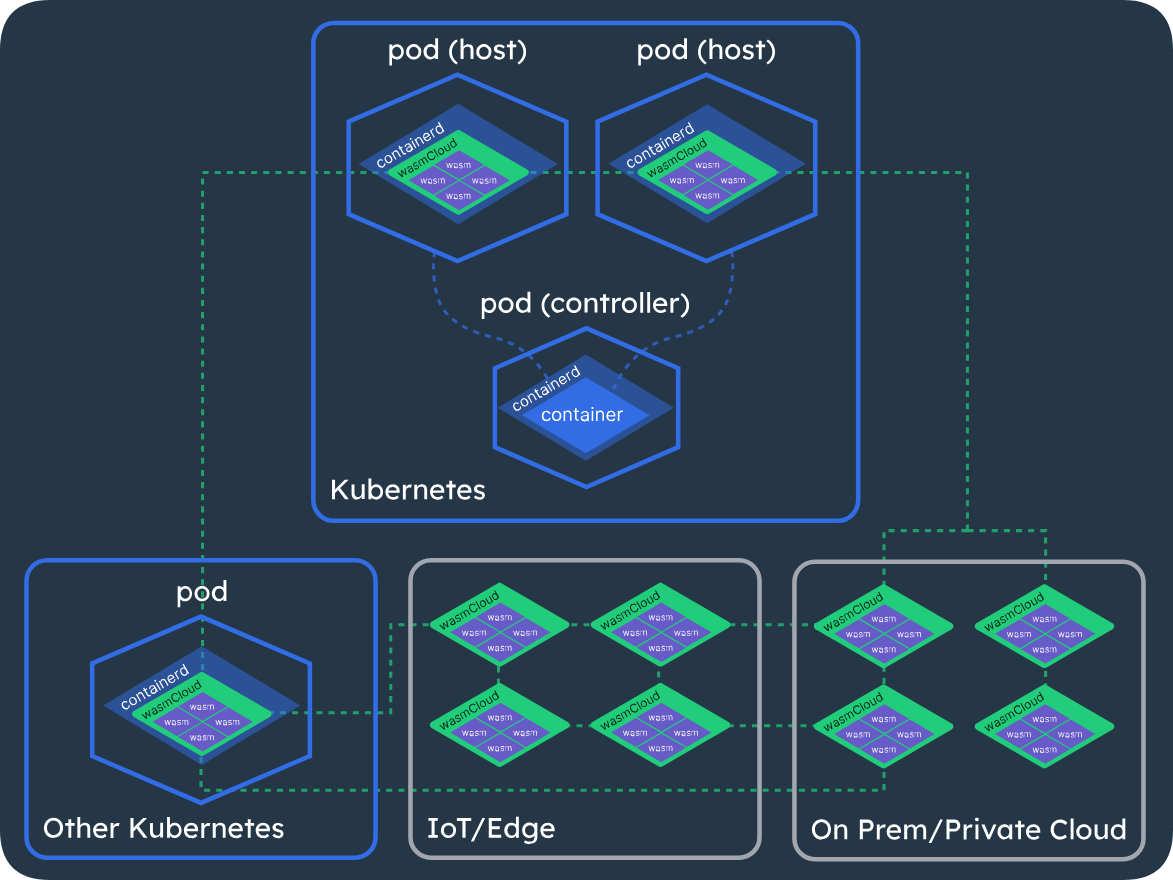
\includegraphics[width=0.8\textwidth]{img/wasmcloud_kube.png}
    \caption{wasmCloud nell'Edge-Cloud Continuum\protect\footnotemark}
    \label{fig:wasmcloud_edge}
\end{figure}
\FloatBarrier
\footnotetext{\url{https://wasmcloud.com/docs/ecosystem/wadm/model/}}

Grazie a NATS e alla rete Lattice la gestione del cluster è facilitata e resiliente, inoltre la toolchain messa a disposizione consente di buildare e deployare facilmente le applicazioni e di fare uso di Provider già pronti.\\
Nella Figura \ref{fig:wasmcloud_arch} viene mostrato un esempio di deployment di un componente Wasm che fa uso di due providers (HTTP server e Key-Value storage) per ampliare le proprie funzionalità.

\FloatBarrier
\begin{figure}[h]
    \centering
    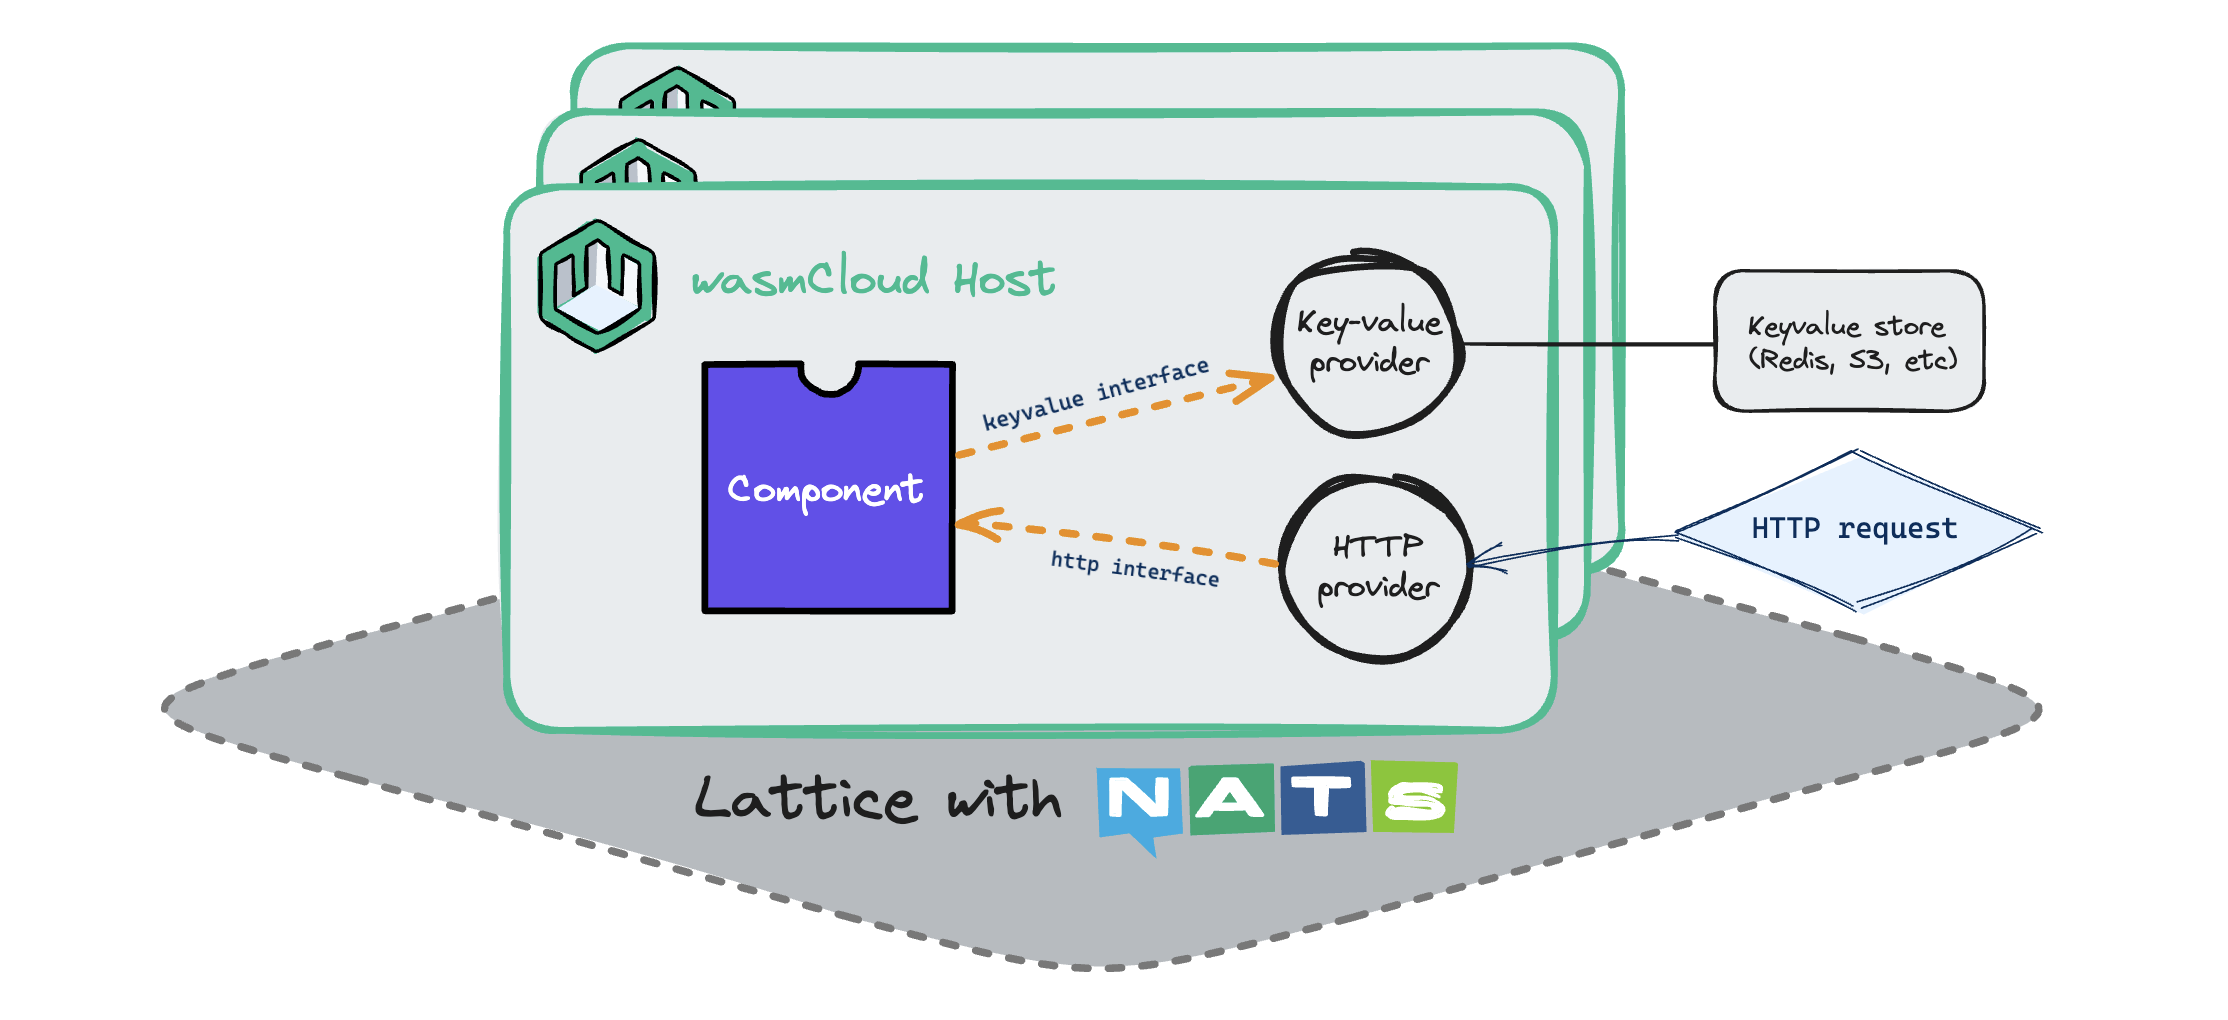
\includegraphics[width=0.9\textwidth]{img/wasmcloud-architecture.png}
    \caption{Architettura di wasmCloud\protect\footnotemark}
    \label{fig:wasmcloud_arch}
\end{figure}
\FloatBarrier
\footnotetext{\url{https://wasmcloud.com/docs/concepts/}}


\section{Related Works}

In questa sezione analizziamo una serie di lavori correlati che hanno contribuito a plasmare il panorama delle tecnologie Cloud ed Edge, fornendo un solido background teorico e pratico su cui basare il nostro studio.\\

\subsubsection{Cloudflare Workers}
In primo luogo, esaminiamo \texttt{Cloudflare Workers}\cite{cloudflare_workers}, una piattaforma serverless che consente di eseguire codice direttamente al bordo della rete globale. Grazie all’adozione del motore V8 e alla capacità di distribuire le funzioni in centinaia di data center in tutto il mondo, Cloudflare Workers rappresenta un esempio paradigmatico di come il FaaS computing possa ridurre la latenza e migliorare la scalabilità delle applicazioni. Recentemente ha introdotto il supporto ai moduli Wasm, integrabili all'interno di funzioni Javascript o eseguibili nativamente con le dovute limitazioni.\\
Sebbene questa sia la soluzione che più si avvicina agli scopi di questo progetto, conferisce un supporto limitato alla tecnologia Wasm, infatti non supporta il modello a componenti e non consente di bilanciare e gestire l'esecuzione dei moduli Wasm fra ambienti Cloud ed Edge\\
Un prodotto interessante è DuckDB-wasm\cite{Kohn2022DuckDB-wasm}, un'integrazione dell'originale DuckDB che introduce web processing asincrono basato su moduli Wasm, incremendando le performance rispetto ad altre librerie diffuse.\\
Fra gli altri lavori non strettamente correlati, ma interessanti per quanto riguarda l'integrazione fra Wasm e l'ecosistema Kubernetes, troviamo \textbf{Spinkube}, già introdotto in precedenza. Questa soluzione mira a fornire un'implementazione dei componenti Wasm all'interno di Kubernetes in modo che possano essere gestiti come semplici container. Questo risultato viene raggiunto tramite un Operator e delle Custom Resource Definition sviluppate ad hoc e ciò permette di deployare degli artifact OCI WebAssembly come Pod.\\
Un altro lavoro interessante è presentato in questo paper\cite{9978884}, che mira ad ottimizzare le performance degli operatori Kubernetes utilizzando un approccio FaaS implementato tramite componenti Wasm e integrazione con WASI. Nella pubblicazione vengono inoltre eseguite delle analisi di performance paragonando i moduli Wasm e i container standard, ottenendo dei buoni risultati.\\
Nel lavoro riportato in questo paper\cite{Nakakaze24}, Wasm viene utilizzato per eseguire Retrofitting (modernizzare un componente/macchinario obsoleto senza rimpiazzarne le parti fondamentali) di dispositivi all'interno di industrie sfruttando le performance e l'isolamento garantite dall'ecosistema WebAssembly.\\
Un altro progetto molto interessante, che è servito come ispirazione per questo elaborato, è quello riportato in questo paper\cite{dcoss}, dove viene proposta una soluzione per distribuire codice tramite messaggi MQTT a dispositivi IoT basata su Wasm.\\

Riassumendo, sebbene siano già presenti prodotti che implementano Wasm con paradigma FaaS e che lo utilizzino per ambienti Edge, non è ancora presente un progetto che unisca i due approcci in un'unica soluzione continuativa e facilmente configurabile anche per un utente poco esperto.
%\section{Papers}

Must read papers: \cite{wiprog}, \cite{Berardi2025ExtremeEdge}, \cite{dcoss}. 
Those are the fundamental papers that support your work. Especifically, \cite{wiprog} and \cite{Berardi2025ExtremeEdge} are well written papers and I highly suggest you to read them to understand how to correct structure a manuscript (introduciton, architecture, implementation and performance evaluation). Further, they are highly related to your work. The work \cite{dcoss} is not so well writen but was the one that inspired your work. \\


Surveys or Reviews are academic papers that summarizes and organizes recent research results in a compreensively way. It is a great way to understand a new reserach field, what are the main challegnes and what is already resolved. In the case of this paper, I suggest citing the follwoing: \cite{Sangeeta23} provides a review of the usage of webassembly for the edge-cloud continuum (read it!), \cite{Ray23} provides a review of webassembly for IoT (take a look to cehck if there is something interesing, but this is not mandatory), and \cite{Hoque2022} which discuss the potential of WebAssembly for Edge Computing (should read it, it is a magazine, so it is shorter). \\


You can cite \cite{Wallentowitz2022} to support the claim that WebAssembly an interesting candidate for Embedded Systems. Do not need to deeply read it, just scan it. Paper \cite{Borui22} follows the same line, it deploys WASM in constrained edge devices -- but this is overall a better paper. You can also just scanned it. \\

Gareth et. al \cite{Gareth2020} discuss the idea of distributing FaaS over the continuum (it not utilizes WASM). Also, paper \cite{Shihong23} discuss more a less the same topics. \\

Paper \cite{Kjorveziroski2023} goes on the orchestration of WASM in serveless computing. It is very related to your thesis. Take a look. \\

This paper \cite{Nakakaze24} should be cite when discussing the communication issues from edge-to-edge using WASM. Take a look how those guys did it. \\

When saying that WASM can be utilized as a container, cite \cite{10682874}. \\

WASM + K8 \cite{9978884}. \\

Use \cite{WASMSpec24} to cite WebAssembly. \\